\documentclass[a4paper,report]{lifestyle}


\RCS $Revision: 1.10 $
\RCS $Date: 2009-10-09 13:29:51 $
\RCS $State: Exp $



\title{\lifetitle{LifeV Developer Manual}
{G. Fourestey \\  S. Deparis \\ L. Formaggia \\ J.-F. Gerbeau \\ C. Prud'homme }
}
\makeindex
\makeglossary

\pagestyle{fancy}

%%\includeonly{lifev-dev_generalities,lifev-dev_howto}

\begin{document}

\maketitle


\phantom{dummy text}
\vfill
This manual is for LifeV (version 0.1, 8 March 2004), a library for scientific computing specially aimed at fluid-structure interaction and blood flow simulation.

Copyright (C) 2001-2008 EPFL, INRIA, Polytechnico Di Milano.

\tableofcontents

\listoffigures

\listoftables

%
\chapter{Generalities}
\label{cha:generalities}

\section{Scope of the document}
\label{sec:scope-document}

This is a ``working document'' meant to drive the development of the
software library \thelibrary. It is an informal document. All the
people involved in the library development (from now on called the
\emph{authors}) are supposed to freely contribute to its writing.

The major objectives of this document is manifold:
\begin{enumerate}
\item Set up a set of rules regarding program development, coding rules
  and standards, which must be followed by the software developers;
\item Provide the architectural design for the libraries and classes
  to be developed, with a special stress on public interfaces;
\item Provide a subtask subdivision for the work to be done and a
  (possibly accurate) \emph{scheduling}.
\end{enumerate}

\section{Language and nomenclature convection}
\label{sec:lang-nomencl-conv}

%Because of many practical reasons, the document will be written in
%English, or at least the best English the authors can manage.

We will use \texttt{typesetting font style} to indicate parts of
actual computer code or name of variables, types, etc..
\textbf{Boldface} is used to mark portion containing rules which
should be followed during program development and \emph{emphasised}
text to indicate important concepts and nomenclature.

\section{Software Management}
\label{sec:software-management}

%This software is the result of the work of many people working in a
%coordinated fashion, some rules for software management
%must be set and agreed upon. A related problem is how to allow for the most ample discussion
%between the authors and, at the same time, coordinate  software
%production.


The software source, its documentation and all related documents (this
one included) is kept in a repository under revision control
using \ixs{CVS}{versioning}\footnote{CVS stands for Concurrent Version System}.


A web site {\it\`a la} Sourceforge\footnote{\url{http://www.sourceforge.net}} \url{http://cmcsforge.epfl.ch} has been set up to host the source code and help the software management.
It requires that you open an account\footnote{\url{https://cmcsforge.epfl.ch/account/register.php}} there and that you declare your intentions to work on \lifev through an email to the development mailing list of \lifev.
Once you are part of the project, you have access to all the facilities: tracker, task manager, CVS repository, forums, document manager and a few other tools which are very useful if not absolutely essential to such a project.

CVS keywords like \verb!Id! and \verb!Log! should not be included in source files,
they cause many unnecessary conflicts at update/commit time. Use
\verb!cvs log! to get the information given by \verb!Id! or \verb!Log!.

\section{Compiling LifeV}
\label{compile-lifev}

In order to compile \lifev, certain requirements must be met in terms
of compilation tools, and libraries to link to.

\noindent In this document, we shall use \verb+$(top_srcdir)+ (aka \verb+$LIFEV_HOME+) to designate the top level \emph{source} directory
and \verb+$(top_builddir)+ to designate the top level \emph{build}
directory where \lifev has been \emph{configured}(see
sections~\ref{sec:compile-cvs} and~\ref{sec:comp-from-offic}) for a
compilation environment.  \verb+$(top_builddir)+ may be different from
\verb+$(top_srcdir)+, see for example the configure hint in
section~\ref{hint:configure}.

\subsection{Requirements}

\subsubsection{Compilation Environment}
\label{sec:comp-envir}

\lifev depends on a number of tools at compilation time, they are part
of the \ix{autotools} from the GNU
project\footnote{\url{http://www.gnu.org}}.

\begin{itemize}
\item \verb!libtool 1.5!\ixns{libtool}{autotools}
\item \verb!automake 1.7!\ixns{automake}{autotools}
\item \verb!autoconf 2.5x x>=2!\ixns{autoconf}{autotools}
\item \verb!g++-4.0 x>=0!\ixns{g++}{compilers}
\item \verb!a version of \verb mpi!
\item \verb!Trilinos!\ixns{aztec}{algebra} (which depends on \verb!mpi!, \verb!blas! and \verb!lapack!)
\item \verb!libumfpack4 (set of routines for solving unsymmetric sparse linear systems)
\end{itemize}

%\subsubsection{Runtime Environment}
%\label{sec:runtime-env}

%\begin{itemize}
%\item \verb!aztec!
%\end{itemize}

\subsection{Compilation from CVS}
\label{sec:compile-cvs}
You need first to have an account on \url{http://cmcsforge.epfl.ch} and
be part of the \lifev project, see~\ref{sec:software-management}.

\noindent First, you need to checkout \lifev. \ixv{CVS} has
been configured to use \ixv{ssh} and your \verb!ssh! keys to
access the

\begin{verbatim}
export CVS_RSH=ssh
cvs -z3 -d:ext:developername@cmcsforge.epfl.ch:/cvsroot/lifev-parallel co lifev-parallel
\end{verbatim}

then place yourself in the new directory :

\begin{verbatim}
cd lifev-parallel
\end{verbatim}

\noindent Second, you have to generate the compilation environment by typing:
\begin{verbatim}
make -f Makefile.cvs
\end{verbatim}

\noindent Third, you have to execute the script
\ixvs{configure}{autotools}
it will automatically check the availability of the needed components
for \lifev compilation. You type:

\begin{verbatim}
configure --with-trilinos-lib=<your trilinos libs path> --with-trilinos-include=<your trilinos include path> --enable-opt --with-openmpi --prefix=<your lifev library install path>

\end{verbatim}

\noindent Finally, you just have to use \ixv{make} to compile \lifev libraries. You type
\begin{verbatim}
make
make install
\end{verbatim}
Optionally, you use \verb!-j x(x=2,3 or 4)! to speed up the compilation time.

\begin{hint}{Configure}
  \label{hint:configure}
  \verb!configure! is extremely powerful and allows you to maintain
  several concurrent build directories. Typically during development
  and testing, you need to have \lifev compiled with debugging flags,
  optimization flags and/or profiling flags. However combining
  optimization and debugging flags does not necessarily produce
  anything useful for debugging and testing purposes.

  With configure it is possible to compile a code in a directory which
  is different from the source directory. This is extremely useful to
  tacke our problem. Let's consider given the source directory to be
  store in the environment variable \verb!$LIFEV_HOME! which is not
  mandatory.

Here is what you can do to compile with debugging flags:
\begin{verbatim}
cd $LIFEV_HOME
mkdir debug
cd debug
CXXFLAGS="-g3 -O0" ../configure
make
\end{verbatim}
Here we have \verb+$(top_builddir) == $LIFEV_HOME/debug+.

Here is what you can do to compile with optimization flags:
\begin{verbatim}
cd $LIFEV_HOME
mkdir optimized
cd optimized
CXXFLAGS="-O2" ../configure
make
\end{verbatim}
Here we have \verb+$(top_builddir) == $LIFEV_HOME/optimized+.

\noindent Note that you may have several concurrent \verb+$(top_builddir)+

\noindent Note that \verb!configure! will fail if you have already compiled
\lifev in the source directory.


\end{hint}


\subsection{Compilation from Official Distribution}
\label{sec:comp-from-offic}
The \lifev project provides releases, they are named using the following convention:
\begin{center}
\verb!lifev-x.y.z.tar.gz!
\end{center}

Here is what you have to do:

\begin{enumerate}
\item download \lifev release \verb!lifev-x.y.z.tar.gz!
\item unpack it
\begin{verbatim}
tar xzf lifev-x.y.z.tar.gz
\end{verbatim}
\item configure it
\begin{verbatim}
cd lifev-x.y.z
configure
\end{verbatim}
\item compile it
\begin{verbatim}
make
\end{verbatim}
\end{enumerate}

Some comments in section\ref{sec:compile-cvs} apply also here.

\subsection{Compiling Testsuite}

\noindent \lifev comes with a testsuite covering a lot of features. It is located in the directory \verb+testsuite+
\begin{verbatim}
|-- data
|-- test_bdf
|-- test_darcy
|-- test_essentialbc
|-- test_fe
|-- test_fsi_newton
|-- test_fsi_picard
|-- test_linearelasticity
|-- test_matrix
|-- test_mesh
|-- test_robin
|-- test_naturalbc
|-- test_ns_bdf
|-- test_ns_cyl
|-- test_ns_sstress
|-- test_p2
|-- test_postproc
`-- test_q1
\end{verbatim}

\noindent In order to compile the testsuite, you need the following steps
\begin{verbatim}
cd $(top_builddir)/testsuite
make check
\end{verbatim}

\noindent If you just want to compile a specific test, say \verb+test_darcy+:
\begin{verbatim}
cd $(top_builddir)/testsuite/data
make check
cd $(top_builddir)/testsuite/test_darcy
make test_darcy _OR_ make check
\end{verbatim}

\noindent Since most tests are using meshes that are located in
\verb+$(top_srcdir)/testsuite/data+, it is mandatory to execute \verb+make check+ in
\verb+$(builddir)/testsuite/data+ in order to create the proper
symlinks to the meshes when \verb+$(top_builddir) != $(top_srcdir)+.

%
%%%%%%%%%%%%% Some Settings for emacs and auc-TeX
% Local Variables:
% TeX-master: "lifev-dev"
% TeX-command-default: "PDFLaTeX"
% TeX-parse-self: t
% TeX-auto-save: t
% TeX-auto-regexp-list: TeX-auto-full-regexp-list
% eval: (ispell-change-dictionary "american")
% End:
%

%\include{lifev-dev_examples}
\chapter{Program Development Conventions} 

\section{Documentation Rules} 


All classes and methods should have
documentations lines which explain in a concise but thorough way it
usage. Documentation should be provided  with methods
\emph{declarations}

The amount of information contained in the documentation of functions
and methods should augment in the following order (unless there are
special needs)
\begin{itemize}
\item Inlined private methods, constructors and destructor;
\item Inlined methods;
\item Public methods;
\item User interface methods.
\end{itemize}
By \emph{user interface methods} we intend those methods that are
meant to be directly called by the user of the library. Those methods
should be the best documented.

\subsection{Methods and function documentation}
\label{sec:fdoc}
I present a template for documentation of a method, which is meant to
serve as example.


\begin{verbatim}

void Euler::Gudonov(Real nflux[4], Real const lsol[4],
                    Real const rsol[4], Real const & nx,
                    Real const & ny)
{
/*
  #Version  1.0. Released 1/1/99. Marco Manzini 1999

  #Purposes: Computed Gudonov numerical fluxes
   (This part describes what the routine does)

  #Input: lsol  -> left state   (density, ux, uy, pressure)
          rsol  -> right state  (,,)
          nx,ny -> references to the 
                   outward oriented components of normal of control volume
   (This part describes the input 
  
  #Output nflux -> numerical fluxes

  #Preconditions: lsol and rsol, should be valid states. 
                  nx*nx + ny*ny =1   

  #Preconditions Tests
                  Euler::ok.state should be used for the validity check of 
                  lstate and rstate.
                  
                  
  #Postconditions: nflux returns the numerical flux according to Gudunov
                   method. 

  #Postcondition Tests Not provided


*/
\end{verbatim}

In the documentation we provide a few keywords, identified by \verb!#!.
\begin{description}
\item The \emph{Version} keyword introduce a comment line which
  contains a reference number and \emph{DATE} which could be used to
  identify the revision of the routine we are using. This is
  particularly important for functions whose implementation may
  change. In particular, The keywords \emph{experimental}, and
  \emph{validated} should be respectively used to indicate software
  still on the experimental stage (no extensive validations made), and
  software already validated by tests. The name of the principal
  author should appear as well.
\item The \emph{Purposes} keyword introduces a brief description of
  the function scopes. Without establishing hard rules, the details
  contained in this part should increase the more the function usage
  is complex, the more it is near to the ``final user'' (in particular
  a detailed description should be done of user interface functions).
  In addition, it is expected that this part should be more carefully
  written in case of \emph{validated} software than
  \emph{experimental} one.
\item The \emph{Input} keyword introduces the description of the
  input arguments. A constant input argument is an argument which is
  \emph{never} modified by the function. Whenever a constant input is
  passed by reference it \emph{should be indicated by the C++ keyword
    \texttt{const}, i.e.\  it should be made a constant reference}. This
  help both the user and the compiler. Some routines may take
  additional input data from a file (or in general from an input
  stream). In that case, details should be indicated in this section.
\item The \emph{Output} keyword introduces a brief description of
  the function outputs, which may be  manifold:
  \begin{enumerate}
  \item A non-constant reference argument (note that a non-constant
    reference may be also an input, in that case its description will
    be repeated in the input section);
  \item A return value for the function;
  \item An output stream.
  \end{enumerate}
\item The \emph{Preconditions} keyword contains the conditions the
  input should satisfy in order to be proper. In particular the
  \emph{Preconditions Tests} section contains the lists of methods
  which should be used to verify if the preconditions are satisfied.
  The preconditions test \emph{should be automatically activated if
    the compiler switch \texttt{-DTEST\_PRE} has been used} (see
  section on debugging).
\item The \emph{Postconditions} keyword contains the conditions the
  output should satisfy in order to be proper.In particular the
  \emph{Postconditions Tests} section contains the lists of methods
  which should be used to verify if the postconditions are satisfied.
  The postconditions tests \emph{should be automatically activated if
    the compiler switch \texttt{-DTEST\_POS} has been used} (see
  section on debugging).
\item Array bounds checking is switched on by the \texttt{TEST\_BOUNDS} switch.
\end{description}
\subsection{Class documentation}
\begin{verbatim}
class FiniteElement : public GenericFiniteElement
{
/*
  #Version  1.0. Released. Giulio Cesare 89 A.C.

  #Purposes: This class contains an implementation of the SPQR finite
             elements.

  #Public data:
   
  #Private data:
           
  #Invariants                

  #Invariant Tests
                  

*/
\end{verbatim}
\begin{description}
\item The keyword \emph{version} has the same meaning as for the 
case of a function.
\item \emph{Purposes} is used to introduce a brief but exhaustive
description of tha class scopes.
\item \emph{Public Data} introduces a description of any public
data which the class contains, in particular static data.
\item The keyword \emph{Private data} should contain a description of
  the private data. It is used to give information to a potential
  programmer of the class. Thus it is required only for classes which
  are likely to be modified and for public data whose description if
  felt necessary for a clear understanding of the algorithms
  implemented in the classes method.
\item The keyword \emph{Invariants} tags the description of the
  class invariant quantities. These are properties that the class
  public and private data should satisfy if the class is in a correct
  state.  For instance, one may impose that each instance of the class
  \emph{Positive\_Definite\_Matrix}, used for positive definite
  matrices, should satisfy the condition that the minimum eigenvalue
  of the stored matrix is positive.
\item One may than devise a test, which will be a class method and
  will be described under the sub-item \emph{Invariants tests},
  which verify that condition. The test should be used for debugging
  purposes and activated when the compiler flag \texttt{-DTEST\_INV} is
  switched on (see section on debugging).
\end{description}

\subsection{File documentation}
Since class and methods are declared in a \texttt{.h} file, the first
line of the file will contain as well some of the documentation.
In particular the \emph{Version} and the  \emph{Purpose} field.
For the \emph{Version}  field, we will follow the convention that
\begin{itemize}
\item If a class does not contain it, the value of the file
containing the class is used;
\item If a function description does not contain it and the function
is a method, the one of the class applies, otherwise that of the file
containing the function declaration.
\end{itemize}

% 
\section{General Nomenclature and Programming Convention}
\subsection{Coding Standards}
We will follow the following simple rules:
\begin{itemize}
\item All declaration in \texttt{*.h} files. Method definitions (a part
  inlined methods or other possible special cases) are in a
  \texttt{cc} file with the same name;
\item No inlined methods definition within classes declarations, unless
they are \textbf{VERY} short. Inlined methods will be defined 
immediately after class declaration.
\item Use \texttt{INLINE} macro, instead of \texttt{inline}. The
  inline macro is switched off if \texttt{-DNOINLINE} is used.
\item Variables and classes must have names which recall their usage.
  Public variables named \texttt{a} or \texttt{pippo} are forbidden.
\item Class name have their first letter UPPER case, if the
    name is formed by many ``words'' the word initial letter is also
    upper case.  Ex.: \texttt{class MySimpleArray}.
\item \emph{Public} variables and functions names follow the same rule
as class names, a part from teh fact that the first letter is \emph{always} lower case. Example: \emph{Real pressure}, \texttt{Matrix \& computeMassMatrix(FiniteElement const \& localElement)}
\item Avoid function declarations without argument name. 
That is
\begin{verbatim}
Matrix & computeMassMatrix(FiniteElement const & localElement);
\end{verbatim}
should be used instead of
\begin{verbatim}
Matrix & computeMassMatrix(FiniteElement const & );
\end{verbatim}                                
This greatly helps understanding how the function works.
\item Use \texttt{const} keyword when possible. It helps the compiler
  and the human being reading the code. Moreover, it enhance
  debugging.
\item Typedefs aliases name follow the same rule as classes names.
\item Use the typedefs aliases \texttt{Real}, \texttt{Int} and
  \texttt{Uint}, instead of the in-built types \texttt{float},
  \texttt{Int} and \texttt{unsigned int}.  It helps making code
  changes afterwards. 
\item C preprocessor macros name are ALL UPPERCASE.
\item All principal classes will have a method
\begin{verbatim}
void  showMe(ostream & logStream);
\end{verbatim}
  which output on \texttt{logStream} (which may be the standard output
  or a file)  the state of the class (i.e.\  the content of the global
  and local variables.  Example (to be verified)
\begin{verbatim}
class AStupidArray {
public:
void addToArray(Real const & value);
...
void  showMe(ostream & logStream);
private  
_myArray[4][4];
}
void AStupidArray::showMe(ostream & logStream)
{
for(int i =0; i<4; ++i)
 {
   for(int j =0; j<4; ++i)
    logSteam << ''_myArray['' << i << '','' << j << ''] ''<<_myArray[i][j]<< endl;
 }
}
\end{verbatim}
\end{itemize}
We will also folly the coding practices outlined in the document
\textbf{Coding Standards} elaborated by \emph{The Laboratory for
  Scientific Computing, University of Notre Dame}, available
searching the Lab home page at \texttt{http:///www.lsc.nd.edu}.
                                
%
\section{Static and dynamic polymorphism}
%

% 
\section{Standard Template Library}
%
\subsection{Containers} We will make extensive use of STL containers
(in particular vectors and maps). This especially in the mesh handler.
\subsection{Strings}
%
We will use STL strings classes, much more flexible than C-style
strings.
\subsection{valarray}
%
\texttt{valarray} class is still not available in gnu c++. Then we
will avoid it for the moment. Yet, we will consider its adoption when correctly implemented in g++.
%
\section{Namespaces}
%
Still too early, but we suggest to read the C++ reference manual. They
may be of help to avoid name clashing in the future.
%
%
\section{Debugging and assertions} 
% 
\section{Debugging}
Debugging is essential! 
In the following we address the following issues
\begin{itemize}
\item Usage of \texttt{assert}s;
\item Usage of \texttt{cpp}  \texttt{-D} compiler switch for
switching on/off debugging at different level;
\item Usage of \texttt{cpp} \texttt{define}s to implement useful
macros and reduce typing (and typing errors!);
\item Debugging inlined functions.
\end{itemize}
\subsection{Assertions}
Assertion is a way of control the satisfaction of certain conditions.
If the condition is not satisfied an error message is printed and the
program is aborted.  

The C header file \texttt{assert.h} provide some basic utilities for
assertion, in particular the command \texttt{assert(b)}, will abort
the program if $b=0$ (i.e.\  false) giving an indication of the file and
the line where the assertion has failed. The \texttt{assert} is in
fact a \texttt{cpp} macro which can be turned off by setting the
compiler switch \texttt{-DNDEBUG} (NOT debug). It is rather crude,
thus we propose something similar but more sophisticated, following what
has been done by E.Berolazzi and M.Manzini in the \texttt{P2MESH} Library.
We define the following set of macros:

\begin{tabularx}{\textwidth}{|l|X|}
  \hline \texttt{ERROR\_MSG(A)} & Basic error message handler, used by
  all other macros.  It is NEVER switched off. It prints the stream
  \texttt{A} (which may be a string of something more complex) on the
  standard error \texttt{cerr} stream, lus an indication of the line and
  file where the condition occurred,
  and aborts the program.\\
  \texttt{ASSERT(X,A)} & Verifies condition \texttt{A} (which will be
  a logical expression), if not satisfied it will abort the program,
  writing the stream \texttt{A} plus an indication of the line and
  file where the condition occurred. It is switched \textbf{off} ONLY
  if
  \texttt{-DNODEBUG} is used at compile level. This should be used for the basic error checks that we would normally let active.\\
  \texttt{ASSERT\_PRE(X,A)} & Specialised \texttt{ASSERT} for
  \textit{preconditions} (see documentation section). It is switched
  \textbf{on} ONLY if \texttt{-DTEST\_PRE} of \texttt{-DTEST\_ALL} is
  used at compilation time.\\
 \texttt{ASSERT\_POS(X,A)} & Specialized \texttt{ASSERT} for
  \textit{postconditions} (see documentation section). It is switched
  \textbf{on} ONLY if \texttt{-DTEST\_POS} of \texttt{-DTEST\_ALL} is
  used at compilation time.\\
 \texttt{ASSERT\_INV(X,A)} & Specialized \texttt{ASSERT} for
  \textit{invariants} (see documentation section). It is switched
  \textbf{on} ONLY if \texttt{-DTEST\_INV} of \texttt{-DTEST\_ALL} is
  used at compilation time.\\\hline
\end{tabularx}

The last three asserts allow to modulate testing of pre, post
conditions and invariants. \texttt{ASSERT} macro have a \texttt{0}ed
version (e.g. \texttt{ASSERT0(X,A)}) which is never turned off.  An
example
\begin{verbatim}
bool complicatedCondition(const Matrix & A);
.....
.....
ASSERT(a>0,''The quantity a should be positive. Instead it is equal to ''<< a) ;
....
....
ASSERT_PRE(complicatedCondition(B),''Precondition test on matrix B not satisfied'') ;
...
...
\end{verbatim}
The \texttt{ASSERT}'s macros (c preprocessor macros) are defined in
the \texttt{lifeV.h} file. (YES, until somebody else give me another
name, I will call the software \textit{lifeV}, in memory of the all
\textit{life}s experienced in the past (I skipped III and IV, just for fun).

\subsection{Compiler Switches and define's}
\begin{itemize}
\item \texttt{-DTEST\_BOUND}  switches on bound checking in all
  arrays-like structure used in the library.
\item\texttt{-DTEST\_PRE} Preconditions are checked.
\item\texttt{-DTEST\_INV} Invariants are checked.
\item\texttt{-DTEST\_POS} Postconditions are checked.
\item \texttt{-DNOINLINE} switches of all \texttt{INLINE} macros.
  \texttt{INLINE} macros should be used in place of \texttt{inline}, in
  order to be able to switch off in-lining during debugging (in-lining
  makes debugging more complicated).
\item\texttt{-DTEST\_ALL} Equivalent to \texttt{-DTEST\_BOUND -DTEST\_PRE -DTEST\_INV
    -DTEST\_POS -DNOINLINE}
\item \texttt{-DSAVEMEMORY} Does not explicitely store some arrays, but rebuild the information
each time needed. It saves some memory at the expense of computional time.
\item  \texttt{INT\_BCNAME} Uses as name for BConditions just an integer and not
  a string. It saves memory at the expense of a more cryptic program.
\end{itemize}

\section{Type nemas, typedefs and template arguments}

It is very important to follows the convention for Type and Template
Arguments names. C++ allows to give alias to typenames with the
instruction \texttt{typedef} and this is a very useful practice, in
particular if \textbf{a common set of names is constantly used} which
correspond to a clearly identified set of classes. Before recalling the
main Types and setting up their general use we wish to recall some basic 
facts.

$\bullet$ Public typedefs are inherited.

Example
\begin{verbatim}

 class a {
public:
        typedef float Real;
 ....
};

class b: public a
{
....
};
\end{verbatim}

Now,  \verb!b::Real! is in fact a \texttt{float}!
   \medskip

$\bullet$ It is a good practice to expose with a typedef the main
  template arguments of a class template. 

Example: 

\begin{verbatim}
template<typename GEOSHAPE>
class AFiniteElement{

public:
        typedef  GEOSHAPE GeoShape;
........
};
\end{verbatim}

So that it os possible to do
\begin{verbatim}
typedef AFiniteElement<Tetra> ATetraElement;


int main()
{
        ATetraElement pippo;
        ATetraElement::GeoShape theShape;
}
\end{verbatim}
In this way the user does not have to remember the actual definition of
\texttt{ATetraElement} to access the typename of the Basic Geometric
Shape.

Remeber that a special care should be used when a templete class is
derived by a template argument:

\begin{verbatim}

class ABaseClass
public:
typedef Triangle GeoShape;
typedef std:complex<float> Complex;
...
};

template<typename BASE>
class Derived: public BASE
{
public:
  typedef BASE Base; // I expose the templete argument

// I need this since GeoShape is USED in the definition of this class

  typedef typename BASE::GeoShape  GeoShape; 
  Geoshape a; // Here I use GeoShape
};

int main()
{
 Derived<ABaseClass> pippo;
 Derived<ABaseClass>::Complex a; //OK
 Derived<ABaseClass>::GeoShape b; //OK
 .....
}
\end{verbatim}

I do not need to make visible the type \texttt{Complex} inside the
\texttt{Derived<BASE>} class templete since it is not used in the
definition (and I can rely to have it available by inheritance when I
instantiate the template class), I need instead to use the \texttt{typedef
  typename} declaration for \texttt{GeoShape} since it is used inside
the definition of \texttt{Derived<BASE>}.

SONO QUI

complicated by the fact that often the template argument name is the
same of the tepedef I would like to expose. For instance (an example
...) this WILL NOT WORK

template <typename GeoShape>
class FE{
typedef GeoShape Geoshape;
};

since the typedef will be ambiguous. One will need then change it into
something like

template <typename GEOSHAPE>
class FE{
        typedef GEOSHAPE Geoshape;
};

now it will work and inside the class template definition I can use
GEOSHAPE or GeoShape, more or less equivalently (even if, from a
logical point of view, they are different beasts).

We may decide to indicate all template arguments all upper case, yet
this will require too may changes... so I will just change the ones
which are needed to be changed. I prefer to change the name of the
template argument while having the name of the typedef conforming to the general
rules. After all the template argument name is a dummy, while it is
important to be consistent with the type names!.

To make myself clearer (I hope!) a GeoShape (which is the typename for a
generic Basis Geometric Shape: LinearTriangle for example) will alway
typedef eather as GeoShape (generic name) or FaceShape, EdgeShape etc
(specific names) and NOT as My\_Geoshape or GeoShapeType or something
like that. However, I will momentarily keep (for consistency reason)
also these 'old' typedefs, so to avoid too many incompatibilities. Yet
they should gradually go away.

d) There is a clear difference of style between my programming and that
of Jean Fred (who is more experience in C++ than I, after all). I use a
lot inheritance as a mechanism of building more complex classes from
simpler ones. He prefers typedef containement.

I.E.

I would have written (is just an example, it does not correspond to an
actual class of the library!!!)

template<BASISFCT,GEOMAP,Quadrule>
class Fe: public BASISFCT, public GEOMAP
{
public:
typedef BASISFCF BasisFct;
typedef GEOMAP GeoMap;

... etc etc ....
};

while jean Fred prefers

template<BASISFCT,GEOMAP,Quadrule>
class Fe
{
public:
typedef BASISFCF BasisFct;
typedef GEOMAP GeoMap;

... etc etc ....
};

and then access BasisFct and GeoMap interfaces through the typedef.  In
the first case instead, the typedef statement is used only to expose the
template arguments, while the interfaces of BasisFct and GeoMap are
directly available through inheritance.

We may argue for months to what is best and when it is best to use one
strategy or the other... In any case, the existance of both styles in
the library MAKES EVEN MORE IMPORTANT to have a coherent strategy for
type names and typedefs!!!!!

\chapter{General Program Overview} 
\label{cha:gener-progr-overv}

\section{General Typedefs}
\label{s:typedefs}

Some general type definitions for the library are defined in the file
\texttt{lifeV.h} and given a global scope.
They are
\begin{itemize}
\item \texttt{\ix{Real}}.  Float type used for all real variables in the code.
  Normally aliased to \texttt{double}.
\item \texttt{\ix{UInt}}. Integral type that holds non negative values and in
  particular the size of containers.  Aliased to
  \texttt{size\_t} from the Standard Template Library.
\item \texttt{ID}\index{ID} Integral type to use for holding the
  \emph{identifier} of a geometric entity (for instance, a Point, a Face
  etc.). By convention, an identifier of an active entity is always
  supposed to \emph{start from 1}. An active geometric entity is a
  entity which belongs to a \emph{mesh}. The value of the identifier of
  an active geometrical entity \textbf{does} correspond the one plus the
  location of the entity in the \emph{entity container}\index{entity
    container}.
 \end{itemize}
\section{Nomenclature}
A finite element library is a complex piece of software. It is therefore
imperative to set a clear and possibly unambiguous nomenclature.


\centerline{\textbf{Nomenclature List}}
\smallskip

To start with, we will make a clear distinction between
\emph{\ix{Geometric Entities}}, that is an entity
which carry data concerning the geometry, a \emph{Finite Element
  Entity}, which is an entity which carry the data more properly
related to a finite element definition and \emph{Linear Algebra
  Entities}, which are linked to the build up, storage and
manipulation of the final linear system.
\subsection{Nomenclature List}
\begin{description}
  
\item\textbf{Geometric Entity}\index{Geometric Entity} is an object
  that carries data concerning the geometry. Geometric entities are
  \texttt{Point}\index{Point}, \texttt{Vertex}\texttt{Vertex}, a
  \texttt{Edge}\index{Edge}, \texttt{Face}\index{Face} and
  \texttt{Volume}\index{Volume}.
\item\textbf{Geometry Element}. The geometry item of higher phisical
  dimension: a \texttt{Volume} in 3D and a \texttt{Face} in 2D.
\item\textbf{Reference Finite Element}\index{Reference Finite Element},
  is an object carry the data more properly related to a finite element
  definition, in the reference space.
\item\textbf{Mapping}\index{Mapping}, an object that carries data concerning the mapping
  from a \texttt{Reference Finite Element} and the \texttt{Current
    Finite Element.}
\item\textbf{Quadrature}\index{Quadrature} An object that carries all
  knots and weights for quadrature rules on different \texttt{Reference
    Finite Element}.
\item\textbf{Basis Finite Element}\index{Finite Element}. The union of a
  \texttt{Reference Finite Element}, a \texttt{Mapping} and a
  \texttt{Quadrature} form a \texttt{Basis Finite Element}. This is the
  basis for the integration of the various integrals appearing in the
  weak formulation. It has the means to provide the value of the shape
  functions and derivatives at integration points, the Jacobian of the
  mapping, and other finite element related quantities once it is
  associated to a specific \texttt{Geometric Element}.
\item\textbf{Boundary Element}\index{Boundary Element}. The element
  (geometry of finite element) on the boundary of the computational
  domain.
\item\textbf{Current finite element}\index{Current Finite Element}. Is
  is the result of the association of a \texttt{Geometry Element} to a
  \texttt{Basis Finite Element}. It makes available all the quantities
  needed to compute the various integrals on that element. In other
  words, a \texttt{Basis finite element} as such is pretty useless since
  it does not know the actual geometry, yet it provides the methods to
  compute quantities on the current element once it has been provided of
  the geometrical information.
\item \textbf{\emph{Degree of Freedom}}
  (\emph{\ix{Dof!Degree of Freedom}}).  It refer (in a
  general sense) to the coefficient of the finite element expansion for
  a problem variable. It may be either
  \emph{scalar}\index{Degree~of~Freedom!scalar} or
  \emph{vector}\index{Degree~of~Freedom!vector}. A \texttt{Dof} may be
  local to the \texttt{} The Class \texttt{Dof}
  contains also the \texttt{Local-to-global} table.
\item \textbf{Local-to-global}\index{Local-to-global} the
  \texttt{local-to-global} table provides the global numbering of a \texttt{Dof}
  
\item \textbf{\emph{\ix{Node}}}. The ``location'' where a Dof
  is held. It is normally associated with a geometrical entity (but it
  must not be confused with it, it is indeed a Finite Element entity).
  
\item \textbf{\emph{\ix{Vertex}}}. The geometrical entity
  which corresponds to a vertex of a Basis Reference Shape.  The
  number of Vertices of a Geometrical Shape is invariant from the
  mapping. For instance, a \emph{\ix{Linear!Triangle}} and a \emph{Quadratic!Triangle}
  Triangle have both three \emph{\ix{Vertices}}.
  
\item \textbf{\emph{Basis Reference Shape}}\index{Basis Reference
    Shape} (\emph{BasRefSha}). The geometrical shape of the reference
  element. It may be one of the following: \texttt{Point},
  \texttt{Line}, \texttt{Triangle}, \texttt{Quad}, \texttt{Tetra},
  \texttt{Hexa}, \texttt{Prism}.
  
\item \textbf{\emph{Basis Geometric Shape}}\index{Basis Geometric
    Shape} (\emph{GeoShape}). The geometrical shape of the actual
  finite element (for instance \texttt{QuadraticTetra}).
  
\item \textbf{\emph{Basis Geometric Element}} (\emph{MeshElementMarked})
  \index{Basis Geometric Element}. The geometric entity associated to
  a finite element.

\item\textbf{\emph{Element}}. An ambiguous term which may refer either
  to a geometric entity of to the finite element proper. Therefore it
  should be avoided unless its significance its clear from the
  context.
  
\item \textbf{\emph{\ix{Edge}}}. The 1D geometric entity which
  corresponds to a side of a Basis Reference Shape.
  
\item \textbf{\emph{\ix{Face}}}. The 2D geometric entity which
  corresponds to a face of a Basis Reference Shape. In a 2D problem it
  represents the \emph{Basic Geometric Element}.
  
\item \textbf{\emph{\ix{Marker}}}. An user defined attribute which may
  be associated to mesh geometrical entities and which is used to
  store and access problem related data and function, such as a
  boundary condition marker. By default it is just an integer.  The
  marker handling is, at the time being, still a rapidly evolving
  feature.

\item \textbf{\emph{\ix{Volume}}}. The 3D geometric entity
  which corresponds to the \emph{Basic Geometric Element} for 3D
  problems.
  
\item \textbf{\emph{\ix{Point}}}. The 0D geometrical entity
  which fully defines the actual shape of a GeoShape. The Vertices are
  a subset of Points. For instance, a quadratic triangle has 3
  vertices and 6 Points. In the \emph{Local Numbering} of a
  MeshElementMarked, the Points which are also Vertices are numbered first.

\item \textbf{\emph{\ix{Id}}}. Unique identifier (type \texttt{UInt})
for a MeshElementMarked and  Region mesh. 

\item\textbf{\emph{Region Mesh!Mesh}}. The mesh on a
  region of the computational domain formed by basic geometric
  elements of the same type.

\item \textbf{\emph{Field}}.\index{Field} The array holding the Dof
  values. It may be scalar or vector.
  
\item \textbf{\emph{Bare Geometric Entities}}.\index{Bare Geometric
    Entities} Geometric entities (\texttt{BareEdge} and
  \texttt{BareFace}) (see section \text{sec:bareentity}) which contain
  only a minimal set of data and are used internally to build the list
  of edges and faces per Basic Geometric Element.


\end{description}

\section{Paradigms}
\label{sec:paradigms}
Here the  main \textbf{paradigms} that we will follow
\begin{enumerate}
\item The \texttt{MeshElementMarked} is the key entity. All major loops will
  be done on the MeshElementMarked. This is a Finite Element (an possible
  Spectral Element) oriented work;
\item The \texttt{Dof} (degrees of freedoms) are associated to
  geometrical entities;
\item On each element the \texttt{Nodes} are numbered (local
  numbering) following the hierarchy:
\begin{itemize}
\item Nodes on Vertices
\item Nodes on Edge
\item Nodes on Faces
\item Nodes on Volumes.
\end{itemize}
\item Global \texttt{Point}s numbering follow the convention:
\begin{itemize}
\item Vertices first, while Points which are not not vertices have higher numbering.
\end{itemize}
\item Global numbering of the other ``lower dimensional'' items (like
  edges..)  follows instead the rule
\begin{itemize}
\item Boundary items first, while internal item have an higher numbering.
\end{itemize}
\item The Region Mesh always stores the Basic Geometric Elements and
  the Boundary Geometric Elements. For the latter, the local Vertices
  numbering allow to identify the direction of the outward normal. For
  3D problems we follow the right-hand rule, for 2D problems the
  boundary is traversed leaving the domain on the lest (anti-clockwise
  orientation).
\item The global numbering of the degrees of freedom (Dof) follow the
  rule
\begin{itemize}
\item  the first Dof's are those associated to the Vertices (if any);
\item then those associated to the edges (if any);
\item then those associated to the Faces (if any);
\item then those associated to the Volumes (if any);
\end{itemize}
\end{enumerate}

%
\section{Scope of the software}
\label{sec:scope-software}
%
%
The scope of the software is o provide efficient, flexible
object-oriented tools for the development of finite element (and
potentially spectral element) algorithms for fluid and fluid-structure
interaction problems.  In the long term the library should account for
\begin{itemize}
\item 2D and 3D domains;
\item Lagrangian and mixed finite elements;
\item Parametric mapping;
\item Support for spectral elements;
\item Support for domain decomposition approaches;
\item ALE algorithms;
\item Support for parallelisation;
\item Simple structural models;
\item Fluid Structure coupling;
\item Mesh adaption.
\end{itemize}
Since the long term goal would take at least 3 man-years of work, some
short term goals have been set:
\begin{itemize}
\item Porting to object oriented paradigm and reprogramming in C++ the
  existing 2D LIFE library. This task would provide useful suggestions
  for the 3D work and would serve as self-teaching purpose for the
  part of the authors without any experience in C++ coding.
\item Development of the core 3D library with support for P1, P2 and
  iso-P2 elements and coupling with simple structural models.
\item A prototype for parallelisation using existing libraries
  (Aztec).
\end{itemize} 
This short term goals should be accomplished in the time frame of 8
months.

Details in the section \ref{ch:scheduling}.


\section{A top-bottom overview} 
\label{sec:top-bottom-overview}
% 
\marginpar{Here we should put an overview of the library, starting from
  the definition of meshes and domains, down to the FEM classes}
\subsection{Domain, Regions and Meshes}
\label{sec:doma-regi-mesh}

\subsubsection{Generalities}
\label{sec:generalities}

The \emph{\ix{Computations Domain!Domain}} will generally be subdivided into
\emph{\ix{sub-domains!Domain}} which are associated either to a different set of
equations to be solved or to different portions which will be treated
independently, for instance for parallelisation purposes.

In order to avoid ambiguities we refer to \emph{Region} to indicate a
portion of the domain ``homogeneous'' both with respect to the set of
equations to be solved and to the type of discretisation employed.

For instance, we may decide to use Hexa elements in one region and
tetrahedra in another region.

To each region is then associated a \emph{RegionMesh}, which will then
be formed by a \emph{homogeneous} set of ``elements''. The union of the
\emph{RegionMesh}es forms the \emph{Mesh}
\subsubsection{Mesh}
The mesh is a container of RegionMeshes. It will also contain all the
necessary tools to exchange information between the Regions. The
details have still to be sorted out.
\subsubsection{RegionMesh}
A RegionMesh is a container of \emph{geometrical} and
\emph{topological} entities, that is entities which describe the mesh
geometry and its connectivity. Every RegionMesh contains a
\emph{DomainMesh} and a \emph{BoundaryMesh}. That is, all information
on the boundary geometry is accessible separately. Some geometrical
entity will have a \emph{marker}, which in the simplest case will just
be an integer, which will allow to identify boundary conditions and/or
different material properties. Some methods will be available to
create containers (STL maps) of pointers to geometrical entities
indexed by the marker value. This would allow efficient implementation
of the boundary conditions.
% 
\subsection{Finite Elements}

\subsection{Field}
A \textit{Field} is defined on a mesh and on a BasisFinite Element.
The number of degrees of freedom are associated to the various
geometrical entities and the numbering convention we adopt allows for
a easy dimensioning of the field vectors and to local-to-global
numbering association (see section \ref{sec:paradigms}).
\section{Main libraries} 
%
The code will consists of 3 main libraries:
\begin{enumerate}
\item \emph{Mesh handler}. The scope of the library is to read a mesh
  description (in a format still to be discussed) and to build the
  data structures which handle geometry and mesh topology
  informations.
\item \emph{Algebra package} This package will contain all the classes
  for storing matrices and vectors and the solvers. We wish to use
  external produced libraries, thus the following rule should be
  followed:
\end{enumerate}
                                %
%

%
\section{Library header files}
\subsection{The main header file}

The file \texttt{lifeV.h} contains all the definitions and macros shared by all the library.
In particular we report here:
\begin{verbatim}
#define ABORT() abort() // Macro for abort

// debugging macros:
# define ERROR_MSG(A)  \
   do { cerr << endl << endl << A << endl << endl ; ABORT() ; } while (0)

// assert macros
  
# define ASSERT0(X,A) if ( !(X) ) \
ERROR_MSG(A << endl << "Error in file" << __FILE__ << " line " << __LINE__) ;

# define ASSERT_PRE0(X,A) if ( !(X) ) \
ERROR_MSG(A << endl << "Precondition Error " << "in file " << __FILE__ \
            << " line " << __LINE__) ;


# define ASSERT_POS0(X,A) if ( !(X) ) \
ERROR_MSG(A << endl <<"Postcondition Error " << "in file " << __FILE__ \
            << " line " << __LINE__) ;


# define ASSERT_INV0(X,A)  if ( !(X) ) \
ERROR_MSG(A <<endl <<  "Invariant Error " << "in file " << __FILE__  \
          << " line " << __LINE__) ;

# define ASSERT_BD0(X)  if ( !(X) ) \
ERROR_MSG("Array bound error " << "in file " << __FILE__  \
          << " line " << __LINE__) ;

\end{verbatim}
The compiler switches may be used to mask some of the asserts, they
are \texttt{TEST\_PRE, TEST\_POS, TEST\_INV, TEST\_BOUNDS, NOINLINE }.
Their meaning is evident from their name and their relation with
\emph{assertions} is detailed in section (\ref{sec:fdoc}).  We have
defined also a \texttt{TEST\_ALL} compiler switch which turns on all
testings.
`
The \texttt{restrict} C++ keyword is not yet supported by many compilers, therefore it it masked by default. If a compiler has it, you should  indicate \texttt{-DHAS\_RESTRICT}.

Some typedefs:
\begin{verbatim} 
typedef double Real;
typedef int Int;
//typedef unsigned int UInt;
typedef size_t  UInt;
typedef unsigned short int USInt;
\end{verbatim}
Since the library support 2D and 3D problems (and in principle 1D problems) we have set a switch.
\begin{verbatim}
#if defined(TWODIM) && defined(THREEDIM) && defined(ONEDIM)
#error Dont be silly. Either One, Two or Three dimensions.
#endif
#if defined(ONEDIM)
#define NDIM 1
extern const UInt nDimensions=1;
#elif defined(TWODIM)
#define NDIM 2
extern const UInt nDimensions=2;
#elif defined(THREEDIM)
#define NDIM 3
extern const UInt nDimensions=3;
#else error You MUST compile with either -DONEDIM, -DTWODIM of -DTHREEDIM set, sorry.
#endif
\end{verbatim}
The 1D version is, at the moment, there only ``virtually'', since no
1D finite elements have been programmed yet.

\subsection{Basis Geometric Shapes}
\label{sec:basgeosha}
They are contained in the header file \texttt{basisElsh.h}.  We make a
distinction between \texttt{Basis Reference Shapes} (\emph{BasRefSha})
and \texttt{Basis Geometric Shapes} (\emph{GeoShape}). The firsts
represent the basic geometries in the reference space. For instance,
the class \texttt{Tetra}:
\begin{verbatim}
class Tetra
{
 public:
  static const ReferenceShapes Shape=TETRA;
  static const UInt nDim=3;
  static const UInt numVertices=4;
  static const UInt numFaces=4;
  static  const UInt numEdges=numFaces+numVertices-2;
};
\end{verbatim}
These classes contains \textbf{only static quantities}.
In particular

\begin{tabularx}{\textwidth}{lX}
\hline
\texttt{Shape} & an \texttt{enum} variable used to identify the shape.\\
\texttt{nDim}  & the dimension of the geometric figure identified by the class\\
\texttt{numVertices} & Number of vertices\\
\texttt{numFaces} & Number of faces\\
\texttt{numEdges} & Number of edges\\
\hline
\end{tabularx}

At the time being we are effectively supporting only shapes whose
faces are of the same type. The class \texttt{Prism} has not yet been considered,
but its support is planned in the future.
Figure \ref{fig:basrefsha} shows the numbering of vertices, edges and faces
for the Basis Reference Shapes.
\begin{figure}[hbp]
  \begin{center}
    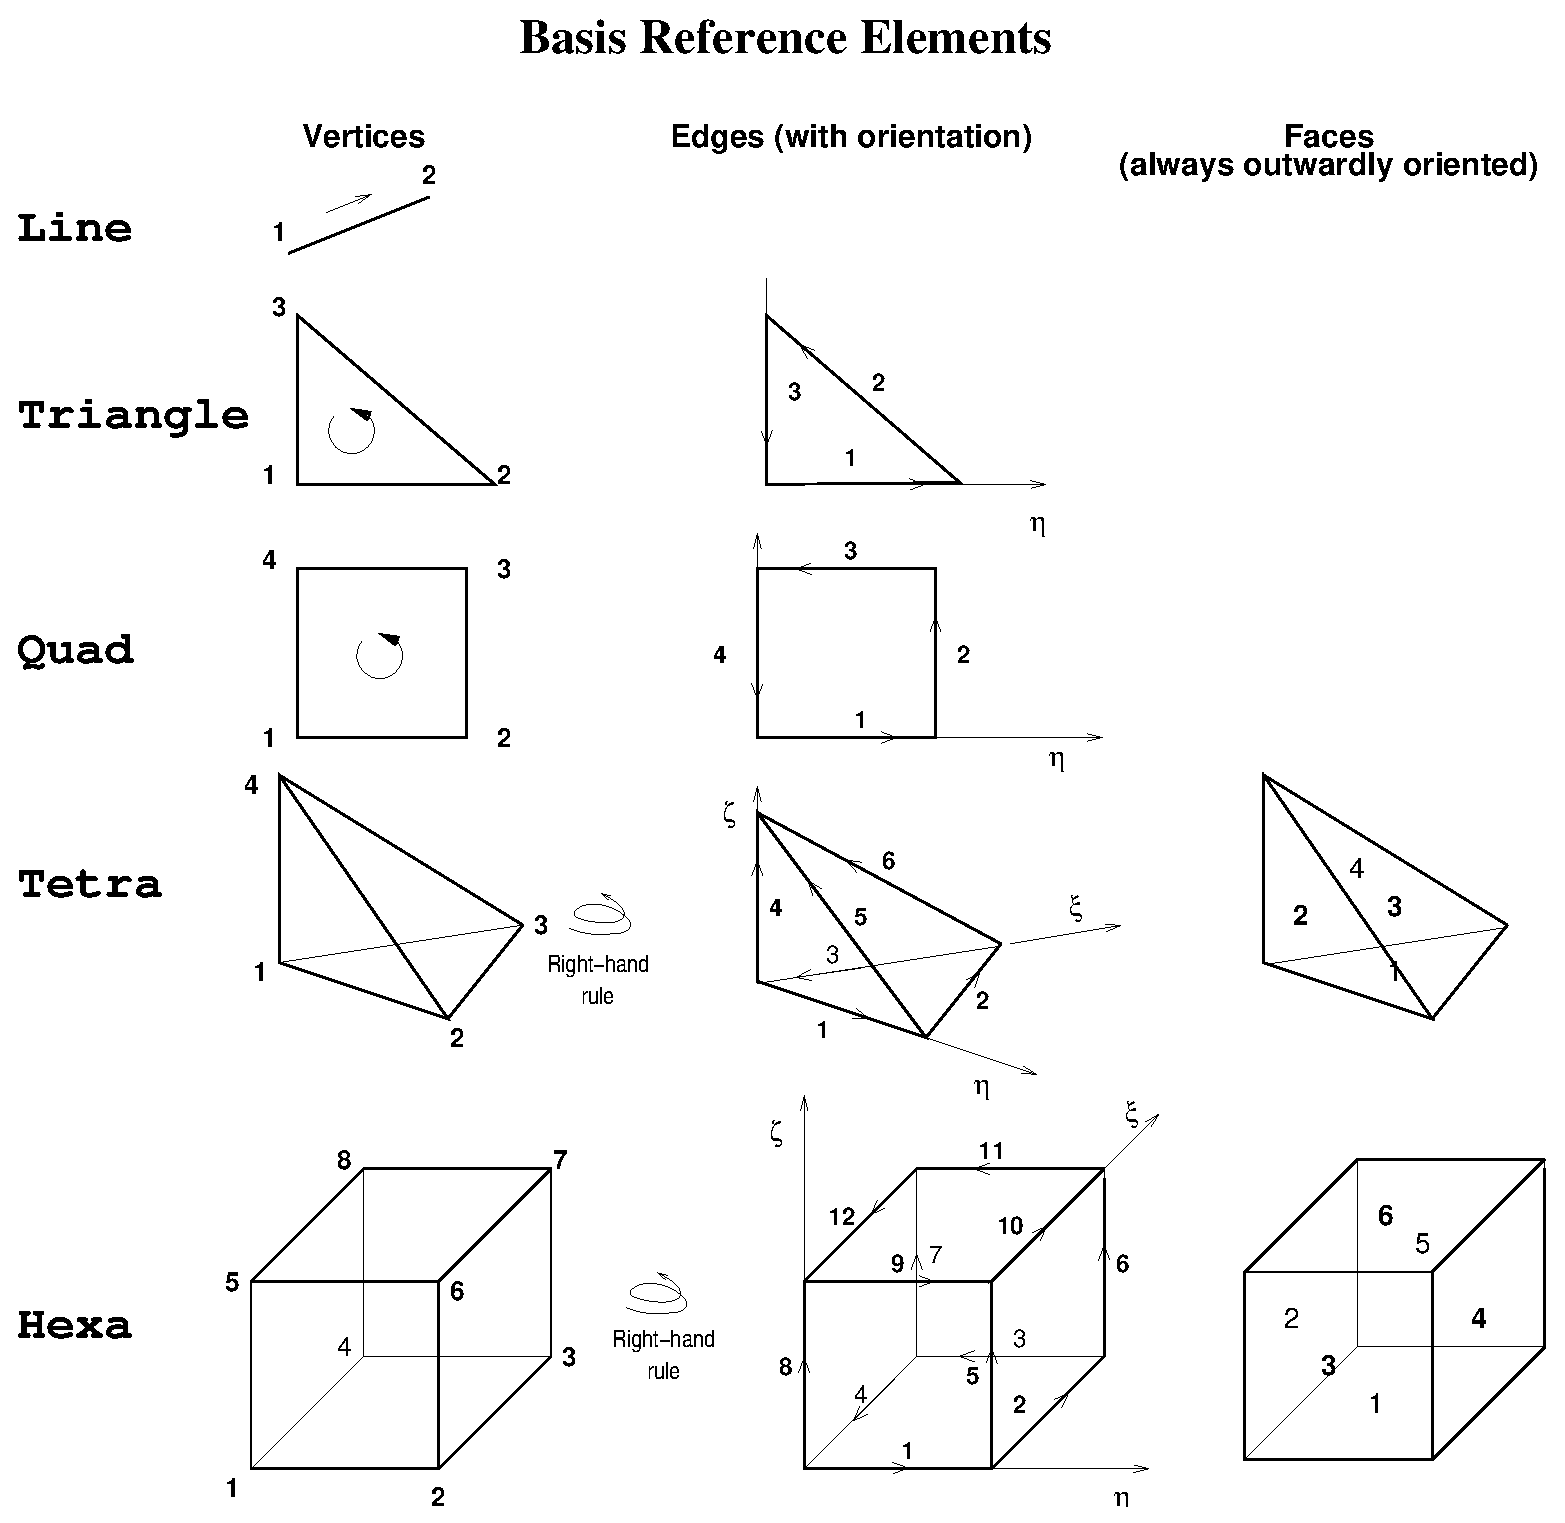
\includegraphics[width=.7\linewidth]{BasElSha}
    
  \end{center}
  \caption{Numbering of vertices, edges and faces
    for the Basis Reference Shapes}\label{fig:basrefsha}
\end{figure}

A \textbf{Basis Geometry Shapes} ia a class derived from a
\emph{BasRefSha}.  It is indeed a specialisation which adds to a
\emph{BasRefSha} additional basic information related to the
\texttt{Points} which will define the shape of the actual geometrical
entity. Again, here we include only the basic information, leaving to
a more specialised class the knowledge of the coordinates of the
points.  An example of \emph{GeoShape} is
\begin{verbatim}
class QuadraticTetra:
public Tetra
{
public:
  typedef Tetra BasRefSha;
  typedef QuadraticTriangle GeoBShape;
  static const UInt numPoints=10;
  static const UInt  numPointsPerEdge    = 1;
  static const UInt  numPointsPerFace    = 0;
  static const UInt  numPointsPerVolume  = 0;
  static UInt edgeToPoint(UInt const _localEdge, UInt const _point);
   static UInt faceToPoint(UInt const _localFace, UInt const _point);
};
\end{verbatim}
Again all data are public and static, due to the basic nature of those
classes (which are in fact \texttt{struct}s).

\begin{tabularx}{\textwidth}{lX}
\hline
\texttt{BasRefSha} & We export the type of the base \emph{BasRefSha}.\\
\texttt{GeoBShape}  & We export the \emph{GeoShape} of the boundary.\\
\texttt{numPoints} & Number of Points\\
\texttt{numPointsPerEdge} & Number of Points \textbf{internal} to an edge\\
\texttt{numPointsPerFace} & Number of Points \textbf{internal} to a face\\
\texttt{numPointsPerVolume} & Number of Points \textbf{internal} to the volume
(i.e.\  to the tetrahedron itself).\\
\texttt{edgeToPoint(i,j)} & $j$-th point on the $i$-the edge (numbering from 1)\\
\texttt{faceToPoint(i,j)} & $j$-th point on the $i$-the face (numbering from 1) \\
\hline
\end{tabularx}

The quantity \texttt{numPointsPerVertex} is not stored because always equal to
$1$. We may note that other pieces of information are immediately deduced. If we take
the example of the Quadratic Tetra we have that the total number of point on each 
face is \texttt{GeoBShape::S_numPoints} while that for the Edges is 
given by \texttt{GeoBShape::GeoBShape::S_numPoints}. The Points numbering follow the
general convention
\begin{itemize}
\item Vertices are numbered first;
\item Then the points internal to edges, following the numbering 
given in figure  \ref{fig:basrefsha};
\item Then the points internal to the faces, again following the numbering 
given in figure  \ref{fig:basrefsha};
\item Finally points internal to the volume.
\end{itemize}
\textbf{Numbering starts from 1}.
Thus, if I want to know the maximum numbering of points on the
edges of a \texttt{QuadraticHexa} I compute
\begin{displaymath}
\text{\texttt{QuadraticHexa::S_numVertices +
QuadraticHexa::S_numPointsPerEdge*QuadraticHexa::S_numEdges}}
\end{displaymath}
\subsection{Mesh Classes}
\label{sec:meshhandler}
The file \texttt{mesh\_handler.h} contains all the remaining information relative to a 
\texttt{RegionMesh} entities.
We start from the Geometric Elements
\subsubsection{Geometric Elements}
The geometric elements are the entities which stores the actual
geometrical information relative to a \texttt{RegionMesh}.  As usual,
they are build by successive specialisation of small modules.  The
first are the \texttt{GeoD} and \texttt{GoeND} classes. The firsts
stores basic information about the actual mesh points. The second is
the base for the build-up of the other, 1d, 2D and 3D  geometric entities.

\begin{verbatim}
class MeshVertex
{
 public:
  
  MeshVertex();
  MeshVertex(MeshVertex const & G);
  MeshVertex & operator=(MeshVertex const & G);

  Real const * coor() const {return _coor;};  
  Real const & x() const;
  Real const & y() const;
  Real const & z() const;
  Real const & coordinate(UInt const i) const;
  
  UInt const & id() const { return _id;}; 
  bool const & boundary() const {return _boundary;};
  void showMe(bool verbose) const;
  
  UInt & id() { return _id;};
  Real & x();
  Real & y();
  Real & z();
  Real * coor() {return _coor;};
  bool & boundary()  {return _boundary;};
  Real & coordinate(UInt const i) ;
};
\end{verbatim}
We give an explanation only of the methods whose meaning is not
obvious.

\begin{tabularx}{\textwidth}{lX} 
\hline 
id() & The unique identifier for the Point, numbering from 1.
  It corresponds to the position in the list of Points in
  \texttt{RegionMesh}. We have both the const and the non-const
  version. I need to find a way to hide the non-const version to the
  general user.  Unfortunately the \texttt{template} arguments limit
  the use of the
  \texttt{friend} operator.\\
  boundary() & True if boundary Point.\\
  showMe(bool verbose) & Throw some info on the standard output. Should be rewritten better.\\
\hline
\end{tabularx}

\begin{verbatim}
template <typename GeoShape>
class MeshElement {
 public:
  
  MeshElement();
  MeshElement(const MeshElement<GeoShape> &);
  MeshElement & operator=(MeshElement const & G); 
  
  static const UInt numLocalPoints=GeoShape::S_numPoints;
  static const UInt numLocalVertices=GeoShape::S_numVertices;
  
  MeshVertex & point(UInt const i); 
  MeshVertex const & point (UInt const i) const;
  
  // UInt const nPoints() const { return GeoShape::S_numPoints; };
  // UInt const nVertices() const { return GeoShape::S_numVertices;};
  
  UInt const & id() const { return _id;}; 
  
  void showMe(bool verbose) const;
  
  void setPoint(UInt const identity, point_Type  const & point); //put point 
  bool setPointWithBoundaryCheck( ID const identity, point_Type const & point ); //with forced bound check
  
  UInt & id() { return _id;};
  
};
\end{verbatim}
The meaning of the variables is quite obvious. \texttt{MeshElement} template class
has a \texttt{GeoShape} as template parameter, since some of its
attribute depend from the geometry of the mesh we are using.

The \texttt{MeshVertex} and \texttt{MeshElement} classes are never instantiated
as such. They are building blocks for the actual
\texttt{MeshElementMarked$n$D} template classes ($n=1,2,3$), which add
attributes more specific to a finite element mesh. The instance of a
\texttt{MeshElementMarked$n$D} template class is what we call a
\emph{Geometry Element}\index{geometry element}, which we generally
indicate as \texttt{GeoEle}.

Here the public interfaces
\begin{verbatim}
template <typename MARKER=PMarker>
class 
MeshElementMarked0D: public MeshVertex, public MarkerHandler<MARKER>
{
 public:
MeshElementMarked0D();
MeshElementMarked0D(MeshElementMarked0D const & g);
MeshElementMarked0D(MeshVertex const & g, MARKER const & m);
MeshElementMarked0D & operator = (MeshElementMarked0D const & g);
};

template 
<typename GeoShape, typename MARKER=EMarker>
class MeshElementMarked1D : public MeshElement<GeoShape>, public MarkerHandler<MARKER>
{
public:
  MeshElementMarked1D();
};

template 
<typename GeoShape, typename MARKER=FMarker>
class MeshElementMarked2D : public MeshElement<GeoShape>, public MarkerHandler<MARKER>
{
public:

  MeshElementMarked2D();

  static const UInt numLocalEdges=GeoShape::S_numVertices;

  typedef typename GeoShape::GeoBShape EdgeShape;
  typedef  MeshElementMarked1D<EdgeShape> EdgeType;
  /* In the 3D case, we store the ids of the adjacent 3Delements.
     NOT THE POINTERS because we don't know the 3Delements type and 
     I don't want to complicate the template declaration */
   ID firstAdjacentElementIdentity() { return M_firstAdjacentElementIdentity;}
   ID secondAdjacentElementIdentity(){ return M_secondAdjacentElementIdentity;}
   ID& firstAdjacentElementIdentity() { return M_firstAdjacentElementIdentity;}
   ID& secondAdjacentElementIdentity(){ return M_secondAdjacentElementIdentity;}
};

template 
<typename GeoShape, typename MARKER=VMarker>
class MeshElementMarked3D : public MeshElement<GeoShape>, public MarkerHandler<MARKER>
{
public:
  
  MeshElementMarked3D();

  typedef typename GeoShape::GeoBShape FaceShape;
  typedef typename FaceShape::GeoBShape EdgeShape;
  typedef  MeshElementMarked1D<EdgeShape> EdgeType;
  typedef  MeshElementMarked2D<FaceShape> FaceType;

  static  const UInt numLocalFaces=GeoShape::S_numFaces;
  static  const UInt numLocalEdges=numLocalFaces+GeoShape::S_numVertices-2;
};
\end{verbatim}
The name of the variables and methods should be self explanatory.
Note the use of the \texttt{DEFINE} C Preprocessor variables
\texttt{TWODIM} and \texttt{THREEDIM} used to identify portion of code
specific to 2D and 3D problems, respectively.  Again, we make an
extensive use of constant \texttt{static} variables for attributes
common to all class members. 

The type of the geometry entity at the boundary is recovered through
the \texttt{GeoBShape} data stored in the \texttt{GeoShape} class. We
need to use the \texttt{typename} keyword to tell the compiler that
the template attributes members are indeed types.

We use the Euler formula to determine some additional information,
such as the number of Edges local to a 3D geometric Element.

The \texttt{MARKER} is a special class used to identify user defined
attributes, such as boundary conditions. It is a still a rapidly
evolving feature, which will be better detailed later on.
\subsubsection{RegionMesh}
Finally, the public interface of a \texttt{RegionMesh} class, which
may be used to hold a 3D mesh.  Here we make large use of
\emph{Standard Template Library} containers (and algorithms). This is
probably the most complex class so far, at least for the part of the
library concerning Mesh and Geometry handling.
Lets look at its public interface piece by piece

\begin{verbatim}
template <typename GeoShape, 
typename MC=MarkerCommon_Base> // Here we will add the Marker_Common class (TO DO)
class RegionMesh : protected MarkerHandler<typename MC::regionMarker>
\end{verbatim}
This is a class template. The second template argument is particular
and its discussion is postponed until te layout of the Marker classes
is more or less at steady state.  We mention only that it contains the
typedefs of all the \texttt{Markers} for all the geometric elements
(the one which have been defaulted to \texttt{PMarker},
\texttt{EMarker} etc.\  in the definition of the \texttt{MeshElementMarked}
classes.  Those types are exported to the \texttt{RegionMesh}, as
usual, in order to be visible at class level without the need of
applying the scope operator on the template argument:
\begin{verbatim}
public:

  typedef typename MC::pointMarker PointMarker;
  typedef typename MC::edgeMarker EdgeMarker;
  typedef typename MC::faceMarker FaceMarker;
  typedef typename MC::volumeMarker VolumeMarker;
  typedef typename MC::regionMarker RegionMarker;
\end{verbatim}

\paragraph{Note By Luca}
We have now the mesh readers, i.e.\  the tools to read a mesh form a file.
Here we have an architectural problem which has not been yet solved.
We had three possibilities
\begin{enumerate}
\item The mesh reader is an external function passed as argument to the 
constructor;
\item The mesh reader is an external function which initialise an empty RegionMEsh object;
\item The mesh reader is a member function.
\end{enumerate}
I have chosen the 3rd alternative, only as a matter of convenience. In
fact, being a member function the reader may directly access the
private members of the class. Of course, this is not a good thing, and
since I took care that all the private member of the RegionMesh can be
indeed accessed by a method of the class, it may be possible to
rewrite the RegionMesh completely as an external module, which is more
safe in case a user wants to add a new mesh reader. I will avoid option $1$
since, although elegant, is a bit messy. $\bullet$

\begin{verbatim}
  bool readMppFile(const string & filename, UInt id, RegionMarker m);
\end{verbatim}
A reader of files in \texttt{mesh++} format.  Now a lot of typedefs
which export to RegionMesh space the types used for the internal data.
\begin{verbatim}

  typedef typename GeoShape::GeoBShape FaceShape;
  typedef typename FaceShape::GeoBShape EdgeShape;
  
  typedef  MeshElementMarked3D<GeoShape,VolumeMarker> VolumeType;
  typedef  MeshElementMarked2D<FaceShape,FaceMarker>  FaceType;
  typedef  MeshElementMarked1D<EdgeShape,EdgeMarker>  EdgeType;
  typedef  MeshElementMarked0D<PointMarker>           point_Type; 

  // Typedefs for STL compliant containers of mesh geometric entities
  // I Use VectorSimple for addressing from 1.

  typedef VectorSimple<point_Type>    Points;  // Point List
  typedef VectorSimple<VolumeType >  Volumes; // 3DElements list
  typedef VectorSimple<FaceType> Faces;       /* Face list:Boundary Faces compulsory,
                                               if needed all faces. */
  typedef VectorSimple<EdgeType> Edges;       /* Edges list:
                                               Filled only if needed, may be empty */
\end{verbatim}  
We use the \texttt{VectorSimple<T>} template class which is a simple
wrap-around to the STL \texttt{vector<T>} template class (see header file
\texttt{VectorSimpleor.h}) to store the list of the various 
Geometrical entities which form the Region Mesh. We follow the following Paradigm
\begin{description}
\item A region mesh stores all the MeshElementMarkeds (Volumes in 3D
  problems, Faces in 2D problems etc), all the Points and all the
  Boundary MeshElementMarkeds. For all the other entities (for instance edges
  in a 3D problem) the storage is done according to a switch which is
  passed to the mesh reader.  Details are still been worked out.
\end{description}

Now we have some methods which return some basic mesh data
\begin{verbatim}
   UInt numLocalFaces() const // Number of local faces for each Volume
   UInt numLocalEdges() const  // Number of local edges for each Volume
   UInt numLocalEdgesOfFace() const //Number of edges on each face
   UInt numElements() const // Total Number of Elements
   UInt numVolumes() const // Total Number of Volumes
   UInt numVertices() const //Total Number of Vertices
   UInt numBVertices() const //Total Number of Boundary Vertices
   UInt numPoints() const //Total Number of Points
   UInt numBPoints() const //Total Number of Boundary Points
   UInt numFaces() const //Total Number of Faces
   UInt numBFaces() const //Total Number of Boundary Faces
   UInt numEdges() const  //Total Number of Edges
   UInt numBEdges() const //Total Number of Boundary Edges
\end{verbatim}
We recall that \texttt{Volume} is the name of a 3D geometry element.
Since \texttt{RegionMesh} handles only 3D problems, we also use the
generic term \texttt{Element} to indicate, in fact, the volumes. That
is we have \texttt{numElements()=numVolumes()}.

Also RegionMeshes have an \texttt{id}:
\begin{verbatim}
UInt const id() const; // Returns id

void showMe(bool verbose); // Prints some mesh info: must be done better!
\end{verbatim}
Now all the methods which allow to access mesh geometric entities
\begin{verbatim}
   point_Type const & point(UInt const i) const; // ith mesh point/vertex
   FaceType const & face(UInt const i) const; // ith mesh face 
   EdgeType const & edge(UInt const i) const; // ith mesh edges  
   VolumeType const & volume(UInt const i) const; //ith mesh 3Delement
   point_Type const & boundaryPoint(UInt const i) const; // ith b. point/vertex
   FaceType  const & boundaryFace(UInt const i) const; // ith b. face.
   EdgeType  const & boundaryEdge(UInt const i) const; // ith b. edge
\end{verbatim}
One must be aware that some of the structures may be only partially
filled up, or even completely empty. It depends on the data we are
actually storing (which depends on the switches which have been set at
mesh construction time (a feature still evolving!)
To help the user, however, here there are some useful methods:
\begin{verbatim}
   bool hasFaces() const;  // Do I store mesh faces?
   bool hasInternalFaces() const; // Do I store also internal faces?
   bool hasEdges() const;         // Do I store edges?
   bool hasInternalEdges() const; // Do I store also internal edges?
\end{verbatim}
Now we recall another \textbf{Paradigm}: points are numbered starting
from the Vertices, the other entities starting from the one on the
boundary.  Yet, we have provided the following methods to interrogate
geometry items (please note that they can take a reference to the
object or its \texttt{id})

\begin{verbatim}
   bool isVertex(point_Type const & p) const;  //Is this point a Vertex?
   bool isBoundaryPoint(point_Type const & p) const;  //Is this point on boundary?
   bool isBoundaryFacet(FaceType const & f) const;  //Is this face on boundary?
   bool isBoundaryEdge(EdgeType const & e) const;  //Is this edge on boundary?
   bool isVertex(UInt const & id) const;  //Is this id a Vertex id?
   bool isBoundaryPoint(UInt const & id) const;  //Is the Point with id on bdry?
   bool isBoundaryFacet(UInt const & id) const;  //Same for a Face id
   bool isBoundaryEdge(UInt const & id) const;  //Same for an Edge id
\end{verbatim}
We now have some stuff which is not set up by default, for memory
reason. For instance, the list of local faces etc. Here are the
methods used to build up and interrogate those structures

We have first a method to get the elements adjacent to a Face. The
method should works if the relative \texttt{Faces} object have been
set up. Therefore, it always works for boundary faces, but not
necessarily for internal faces (which are not set up by default).
 
The method returns the ID of the 3DElement adjacent to a Face.
\texttt{Pos} is an \texttt{UInt} which may be equal to 1 or 2 and it
indicates first or second Element. The first element is the one
\emph{ORIENTED coherently with the face AS STORED in Faces}. It means that
the face orientation is OUTWARD with respect to the element. The second
element is either null (boundary face) or indicates the element where
the face appears INWARD oriented.

\begin{verbatim}
   UInt  faceElement(UInt const faceId, UInt const Pos) const; 
   UInt  faceElement(FaceType const & f, UInt const Pos) const;  
\end{verbatim}

Now we have some other structures which are not set-up by default.  This
are the structures which give the global numbering of an Element local
Faces or Edges. These structures are indeed used for the build up of the
degrees of freedom, but, since they are not always necessary (for
esample, for the setup of the degrees of freedom fro al linear Tetra we
don't need them) we have avoided creating them by default (also because
they eat up a lot of memory).  The actual lists are kept hidden (private
data), the user may only access them through the appropriate
\emph{constant} methods.

  \textsl{Note by Luca: Beware of the fact that the list of local
  faces/edges returns the id of a \texttt{BareFace} (or
  \texttt{BareEdge}) (section \ref{sec:bareentities}). That means that
  an id number is return even if the actual Full \texttt{Face} or
  \texttt{Edge} has \textbf{not} been instantiated and it stored in the
  list of Faces and Edges of the mesh.  This because one may want to
  have a numbering for Faces and Edges (for instance in order to build
  the Degrees of Freedom) without actually creating the corresponding
Full Face or Edge object (i.e. the \texttt{MeshElementMarked2D} and
\texttt{MeshElementMarked1D} object)! Therefore, if the user is interested in
the Full Face of Edge object, he/she must first check whether it exists.
Again, some helper methods are provided to make life a little easier.}

\begin{verbatim}
  bool hasLocalFaces() const; // Is the local Faces array set up?
  bool hasLocalEdges() const; // Same for Edges
\end{verbatim}
There two functions are used to test whether the structures have been set 
up. If not, one may do:
\begin{verbatim}
  void updateElementEdges(); // Build localEdgeId table
  void updateElementFaces(); // Build localFaceId table
\end{verbatim}
Now the methods which return the global nubering of
local faces and edges on a volume element.
\begin{verbatim}
   UInt localFaceId(UInt const volId, UInt const locF) const;
   UInt localEdgeId(UInt const volId, UInt const locE) const;
   UInt localFaceId(const VolumeType & iv, UInt const locF) const;
   UInt localEdgeId(const VolumeType & iv, UInt const locE) const;
\end{verbatim}
Now we may wish to know if a given id correspond to a full edge or
face, that is if the corresponding \texttt{Edge} and \texttt{Face}
objects have been instantiated. 

\begin{verbatim}
bool isFullFace(UInt const & id) const;  //Full data for this face?
bool isFullEdge(UInt const & id) const;  //Full data for this edge?
\end{verbatim}
\subsection{Bare Items}\label{sec:bareentities}
The declarations and definitions of the \texttt{BareItem}s handlers are in
\texttt{bareitem.h}. Since MeshElementBare are used only internally, we are
(temporarily) omitting a detailed documentation. I (Luca) will only
give an explanation of the genesis of the MeshElementBare. The RegionMEsh as
it has been defined is able to store Edge and Face objects. Those
objects are rather complex: they contains a Marker, possibly pointers
to other structures etc. In other words, they use memory and one would
like to avoid to instantiate them if not strictly necessary. Indeed,
the RegionMesh has all the list of edges and faces ready, but in fact,
only the list of boundary faces is filled by default (and probably one
may avoid also that, if needed). 

One of the paradigms chosen for the development of this library is the
fact that degrees of freedom are linked to geometrical entities.  Now
if we have degrees of freedom associated, for instance, to Edges (like
in a P2 Tetra) in order to build the global numbering of the Dof and
the association between local (element wise) and global numbering I
need to identify edges and give them an id number. Yet, maybe I don't want to
build teh Edge object: after all all I need is the numbering and a
way of getting the id's of the point on the edge, all the remaining data 
of the proper Edge object is not necessarily needed. (Beware, that is not anymore true
if I want to associate to some edge associated Dof a boundary condition
different from that of the two adjacent points!. In such case, you need to
have a full edge!).

The dilemma has been resolved by creating the concept of bare edge and
bare face.  A bare item is formed by the minimal information required
to uniquely identify it, namely 2 \texttt{Point}'s \texttt{id} for an
edge and 3 \texttt{Point}'s \texttt{id} for the Faces (it is enough
also for Quad faces!). We build the bare items by looping through the
elements and obviously we make sure that the BareItem \texttt{id} is
consistent with that of the corresponding ``full item'' if the latter
has been instantiated.  There is a little problem with the orientation
of a BareItem on the boundary and the orientation of the corresponding
full entity, which has not yet been fully resolved, but will be done
soon.
\subsection{BC Condition Classes}
The file \texttt{bccond.h} contains the definition of the classes
which are meant to hold boundary condition data. As a matter of fact,
the use of this set of classes may be more general, they may be used,
for instance, to hold domain based data and methods, such the
viscosity function for a fluid flow computation, for instance.
However, in the following we will only refer to the use of these
classes for storing boundary condition data (and methods). Their extension
to other uses is immediate.
We will geneally refer to them as \texttt{BC} classes (and, correpsondingly,
\texttt{BC} objects).

The classes are \emph{estensible}, that is the user may add, by using
the inheritance mechanism, specialised classes derived from the
classes defined in the file. The mechanism here followed to introduce
estensibility is that of \emph{dynamic polymorphism}. By the use of
dynamic polymorphism we have easily designed a container class which
is able to uniformly store the various instances of \texttt{BC}
Classes.

The major classes defined in the files are:
\begin{itemize}
\item A container class, called \texttt{BC\_Handler}. The class is used to store and
retrieve the various instances of \texttt{BC} Classes. It is based on the STL \texttt{set}
container and it effectively stores pointer to \texttt{BC} objects, so it is able
to provide a common uniform interface for base and user defined classes.
\item Two base \texttt{BC} classes, called respectively
  \texttt{BC\_Base} and \texttt{BC\_Base\_WL}. The default and user
  defined classes will be derived from them.  Infact,
  \texttt{BC\_Base\_WL} in inherited from \texttt{BC\_Base} and adds
  to it a vector of unsigned integers. The use of such a vector is to
  possibly store the list of Id's of the items to which that boundary
  condition is associated.
\item Two default \texttt{BC} classes, called \texttt{SimpleBC} and \texttt{simpleBC\_WL},
which are simply inherited form the corresponding base classes.
\item A set of utilities to compare \texttt{BC} objects. Some of this utilities make
use of the RTTI (run time type identification) technique.
\end{itemize}

Before giving more details on  the \texttt{BC} classes, we introduce some nomenclature
which will be used consistently in the following paragraphs.

\paragraph{type} A boundary condition \emph{type} refer to the capabilities of the
boundary condition. Different types will correspond to \emph{different
  classes} (all inherited from a \texttt{BC\_Base}, or
\texttt{BC\_Base\_WL} basis class). The user will create a new type only
if he wants to enucleate some data and methods specific to a
particular boundary treatment.

\paragraph{name} The \emph{name} of a boundary condition. It can be used to find a particular
boundary conditions (if different names are used for different boundary conditions. 


We now detail the various classes.
\subsubsection{BC\_Base and BC\_Base\_WL}
\begin{verbatim}
class BC_Base
{
public:
  virtual void showMe()const;
  template <typename T>
  T& asLeaf(T const _t);
  template <typename T>
  T& asLeaf(T  * _t);
  virtual ~BC_Base(){}
  BC_Base(bcName_Type const _n);
#ifndef INT_BCNAME
  BC_Base(char const * _n);
#endif
  BC_Base();
  bcName_Type & name();
  bcName_Type const & name()const;
  bool unset()const;
protected:
  bcName_Type _name;
};
\end{verbatim}
The class is very simple. It provides methods for explicit dynamic
polymorphism (maybe they are useless). \texttt{showMe()} may be used
for debugging purposes and \texttt{name()} may be used to set the
name. The name may be also given through the constructor. The method
\texttt{unset()} reset the name to the \texttt{nullBCname} value.

The \texttt{BC\_Base\_WL} is just an extension of the
\texttt{BC\_Base} class, with the addition of a STL container of
unsigned integers.
\begin{verbatim}
class
BC_Base_WL: public BC_Base
{
public:
  BC_Base_WL(bcName_Type const _n):BC_Base(_n){};
#ifndef  INT_BCNAME
  BC_Base_WL(char const * _n):BC_Base(_n){};
#endif
  BC_Base_WL():BC_Base(){};
  virtual ~BC_Base_WL(){};
  virtual void showMe()const;
  vector<UInt> idList;
};
\end{verbatim}
\subsubsection{BC\_Handler}
The \texttt{BC\_Handler} is a container of \texttt{BC} polymorphic
objects.  Indeed, it stores a STL set of pointers to \texttt{BC\_Base}
objects. It also provide a set of methods for adding, deleting an
element from the set and for query the set. Furthermore the methods
\texttt{size()} and \texttt{empty()} returns the result of the analog
method applied to the set.

\begin{verbatim}
class BC_Handler
{
public:

  BC_Handler();
  
  typedef typename set<BC_Base *>::iterator   BC_PTR_iterator;
  inline BC_PTR_iterator end()const;
  inline BC_PTR_iterator begin()const;
  int size()const;
  inline bool  empty()const;
\end{verbatim}
The \texttt{BC\_Handler} methods which add/erase an element to the set;
beware that the memory management routine must be done outside: the methods do not
create/erase the \texttt{BC} object, they only operate on the container.

The meaning of method \texttt{showMe()} and of the various overloaded versions
of \texttt{isThere()} is obvious. One may query the set either by giving
a reference/pointer to a \texttt{BC} object, or by giving the name, since no
objects with the same name may be present in the container. 
\begin{verbatim}
  inline bool add(BC_Base  * const _bc);
  inline bool add(BC_Base & _bc);

  
  bool erase_BC(bcName_Type const  _n); /* Deletes entry with name _n
  
  inline bool  isThere(bcName_Type const _n) const;
  inline bool  isThere(BC_Base * const  _p) const;
  inline bool  isThere(BC_Base & _p) const;
  void showMe()const;
\end{verbatim}  

The method \texttt{names()} returns a STL vector with all the names in the 
container.
\begin{verbatim}
  vector<bcName_Type> & names()const;
\end{verbatim}  
\subsubsection{Helper functions}
There are a set of helper function, some of which are quite important.
Two of those are the \texttt{addBC} and the \texttt{addBC\_ptr} template
function, which creates a new \texttt{BC} object and adds it to a
\texttt{BC\_Handler}.  In principle, that function should have been an
\texttt{BC\_Handler} method, but a lack of full compliance with the
treatment of template methods by the current version of \emph{g++}
compiler has made it necessary having \emph{global functions}:

\begin{verbatim}
template
<typename BC=BC_Base>
BC &
addBC(BC_Handler & bh, bcName_Type const _n)

template
<typename BC=BC_Base>
BC *
addBC_ptr(BC_Handler & bh, bcName_Type const _n)
\end{verbatim}

The functions CREATES a new BC object on the memory heap, add it to
the container and return a reference or, respectively, a pointer to
the created object.

The use of the function is immediate and illustarated in the following
example, where both the reference and the pointer version are used.
\begin{verbatim}
// Some userdefined BCs. Just for fun!

class Dirichlet: public BC_Base
{
public:
  Dirichlet(bcName_Type _n): BC_Base(_n)
    {};
  static char* const type="Dirichlet";
  void showMe(){cout << type<< " " <<name()<<endl;}
};

class Neumann: public BC_Base_WL
{
public:
  Neumann(bcName_Type const  _n): BC_Base_WL(_n)
    {};
  static char* const type="Neumann";
  void showMe(){cout << type<< " " <<name()<<endl;}
};

int
main()
{
  BC_Base * pbc;
  BC_Handler Bound_cond; 
  Dirichlet pippo=addBC<Dirichlet>(Bound_cond,"inflow");
  Dirichlet * pluto=addBC_ptr<Dirichlet>(Bound_cond,"wall");
  pluto->showMe();
  pippo.showMe();
  cout << "I am a "<< typeName(pippo)<<endl;
  cout << "I am a "<< typeName(pluto)<<endl;
  Neumann pw=addBC<Neumann>(Bound_cond,"wall");
  Bound_cond.erase_BC("wall");
}
\end{verbatim}
In the previous example we have also shown some utilities which
use the \texttt{RTTI} mechanism to test if two \texttt{BC} objects are 
of the same type, or to query their type. They are
\begin{verbatim}
inline bool sameType(BC_Base const * a, BC_Base const *  t)
inline bool sameType(BC_Base const & a, BC_Base const &  t)
inline bool sameType(BC_Base const & a, BC_Base const *  t)
inline bool sameType(BC_Base const * a, BC_Base const &  t)
inline char const *  typeName(BC_Base const & a)
inline char const *  typeName(BC_Base const * a)
\end{verbatim}
Figure \ref{fig:bchandler} shows a sketch of two \texttt{BC\_Handler}
objects storing two lists of \texttt{BC} objects. 
\begin{figure}[ht]
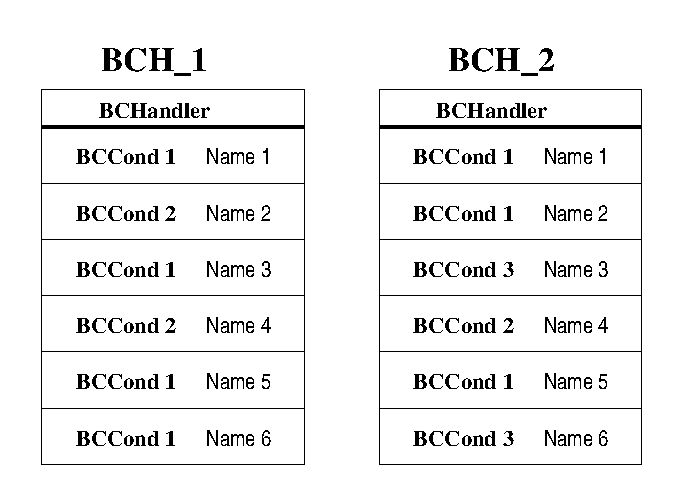
\includegraphics[width=0.8\textwidth]{BCHandler}
\caption{Sketch of two \texttt{BC\_Handler} objects.\label{fig:bchandler}}
\end{figure}


\subsection{Markers}
The \texttt{Marker} classes are at the same time a ``wrapper'' around
the \texttt{BC} class and the tool to be used to extend high level
geometric classes with user defined function and methods. This latter
aspect has been implemented by using the following technique.
x\begin{itemize}
\item A different marker class is defined for each 'high level'
  geometric element (Point, Line etc.). All those classes are in fact
  \emph{extension} (by inheritance) of a basis class, called
  \texttt{Marker\_Base}. \texttt{Marker\_Base} just contains a pointer
  to a \texttt{BC} object and some methods to retrieve it. The user
  may create, \textbf{by inheritance from \texttt{Marker\_Base}}, his
  own marker classes, where he will declare all data and methods which
  he wants to be available to the corresponding geometry element
  class. Indeed, the geometric element class \emph{is derived} from
  the correponding Marker.  Some basic marker classes are provided, to
  which the system defaults if the user does not provide his own.
\item A class template, \texttt{MarkerCommon} takes as template
  parameter the typenames of Marker classes for all geometric
  elements.  The \texttt{MarkerCommon} takes the defaults marker
  classes as default values for the template arguments. The
  \texttt{MarkerCommon} is used as \textbf{mplate argument} for all
  high level geometry classes.  This means, that a pecialised version,
  derived from the basis one, may be used to define \textit{static} data and methods
  the user wants to be available to all high-level geometry entity classes.
\end{itemize}
In conclusion, extension to geometric entity classes is performed by
inheritance from specialised Marker classes. Access to static data an
methods to all geometric entity classes may be done by extending
\texttt{MarkerCommon} (clearly, this is not the only way, global
functions will work as well, but with less ``data hiding'').

In addition, a \texttt{MarkerHandler} class stores the container for
the \texttt{BC} object. The default Marker for \emph{Region} geometric
entities, \texttt(RegionMarker\_Base), id derived from the
\texttt{MarkerHandler} class. This means, that in the default
configuration we have one \texttt{BC} container at the level of a
Region, while the other entities just store a pointer to a \texttt{BC} 
object. The user may change that if necessary.

As usual, some snapshots from the \texttt{markers\_base.h} and \texttt{markers.h}
\subsubsection{\texttt{markers\_base.h}}
Here the \texttt{Marker\_Base} class which stores the \texttt{BC} pointer
and provides the methods to extract it.
The user \texttt{MUST BE WARNED} that in principle a \texttt{Marker\_Base}, and thus
the geometry item which derives from it, may not have a ``boundary condition'' associated.
In order to avoid further complexities, this fact would be accounted by  
having a \texttt{NULL} pointer stored in the \texttt{Marker\_Base} (and thus in the 
corresponding geometric entity). Therefore, some care MUST be taken when 
addressing the \texttt{BC} pointer. That is why the \texttt{MarkerUnset()} method has been provided.

\begin{verbatim}
#include "bccond.h"
class Marker
{
public:
  Marker():_marker(0);
  Marker(BC_Base * const _m ):_marker(_m);
  BC_Base * & marker_ptr();
  BC_Base * const & marker_ptr()const;
  bool markerUnset();
  BC_Base const & marker()const;
  template <typename BC>
  void
  setMarker(BC & _a);
  template <typename BC>
  void
  setMarker(BC  * const  _a);
protected:
  BC_Base * _marker;
};
\end{verbatim}

The \texttt{MarkerHandler\_Base} is just a wrapper for the
\texttt{BC} container.
\begin{verbatim}
class MarkerHandler_Base
{
public:
  MarkerHandler_Base(){};
  BC_Handler & BCList(); \\ returns the list
  BC_Handler const & BCList();
protected:
  BC_Handler _lBC;
};
\end{verbatim}

Here the default marker classes.
\begin{verbatim}
class DefPointMarker: public Marker
{
public:
  DefPointMarker(){};
  DefPointMarker(BC_Base * const _m ):Marker(_m){};
};

class DefFaceMarker: public Marker
{
public:
  DefFaceMarker(){};
  DefFaceMarker(BC_Base * const _m ):Marker(_m){};
};

class DefEdgeMarker: public Marker
{
public:
  DefEdgeMarker(){};
  DeEdgeMarker(BC_Base * const _m ):Marker(_m){};
};

class DefVolumeMarker: public Marker
{
public:
   DefVolumeMarker(){};
   DefVolumeMarker(BC_Base * const _m ):Marker(_m){};
};
\end{verbatim}
The \emph{default region marker} id derived also from
\texttt{MarkerHandler\_Base} class. \emph{In the defaukt layout it is the
region which has the list of boundary conditions.}

\begin{verbatim}
class DefRegionMarker: 
public Marker, public MarkerHandler_Base 
{
public:
   DefRegionMarker{};
   DefRegionMarker(BC_Base * const _m ):Marker(_m){};
};

\end{verbatim}

The \texttt{MarkerCommon} class is used to store the typedefs of the
user defined markers. If the user wants to create his own
\texttt{MarkerCommon} (in order to add data and methods available to all
geometric entities) he has to make a derivation from this one.
The \texttt{MarkerCommon} templates arguments default to the default
Marker classes.

\begin{verbatim}
template
<
class PM=DefPointMarker,
class EM=DefEdgeMarker,
class FM=DefFaceMarker,
class VM=DefVolumeMarker,
class RM=DefRegionMarker
>
class MarkerCommon
{
public:
typedef PM PointMarker;
typedef EM EdgeMarker;
typedef FM FaceMarker;
typedef VM VolumeMarker;
typedef RM RegionMarker;
};
\end{verbatim}

We now define the \texttt{NULLMARKER} as the marker containing an
empty pointer to \texttt{BC} object.  It is useful for testing. An
helper function is provided to test equality of markers (provisional,
may be changed).

\begin{verbatim}
const Marker NULLMARKER=* new Marker; 
inline bool operator==(const Marker & a, const Marker & b);
\end{verbatim}


\subsubsection{\texttt{markers.h}}
This file just contains the type definition of the
default \texttt{MarkerCommon}
\begin{verbatim}
#ifndef HH_MARKERS_HH_
#define HH_MARKERS_HH_
#include "Marker.h"
typedef MarkerCommon<
DefPointMarker,
DefEdgeMarker,
DefFaceMarker,
DefVolumeMarker,
DefRegionMarker
> DefMarkerCommon;
\end{verbatim}

\subsubsection{An example}
Here we comment an example of usage of the default marker classes.

Some user defined \texttt{BC} classes, just for fun!
\begin{verbatim}
#include<iostream>
#include "mesh_handler.h"
class Dirichlet: public BC_Base
{
public:
  Dirichlet(string _n): BC_Base(_n)
    {};
  static char* const type="Dirichlet";
  void showMe(){cout << type<< " " <<name()<<endl;}
};

class Neumann: public BC_Base_WL
{
public:
  Neumann(string const  _n): BC_Base_WL(_n)
    {};
  static char* const type="Neumann";
  void showMe(){cout << type<< " " <<name()<<endl;}
};
\end{verbatim}
Now we declare some geometric entities. Since we use only one
template (the compulsory one which indicates the element basis shape) it
means that we are using the default marker classes.
\begin{verbatim}
  MeshElementMarked1D<LinearLine> line;
  MeshElementMarked2D<LinearTriangle> tri;
  MeshElementMarked2D<LinearTriangle> tri1;
  MeshElementMarked2D<LinearTriangle> tri2;
  MeshElementMarked3D<LinearTetra> tet;
  RegionMesh<LinearTetra> mesh;
  MeshElementMarked0D<> point;
\end{verbatim}

we now define a reference to the boundary condition handler,
which (since we are using the default layout) is an attribute of the
RegionMesh:
\begin{verbatim}
BC_Handler & BCl=mesh.BCList();
\end{verbatim}

Now some examples of different ways of creating/assigning a boundary condition
marker and storing/retrieving  it to/from  the list
\begin{verbatim}
  line.setMarker(addBC<Dirichlet>(BCl,"inflow"));
  tri.marker_ptr()=addBC_ptr<Dirichlet>(BCl,"inflow");
  tri1.marker_ptr()=addBC_ptr<Neumann>(BCl,"outflow");
  tri2.marker_ptr()=addBC_ptr<Neumann>(BCl,"outflow");
\end{verbatim}
\subsection{The pattern classes}
\label{s:pattern}\index{Pattern Classes}
The \texttt{pattern.h} file contains the definitions of the classes
which are able to held the \textbf{pattern} of a global finite lements
sparse matrix. A set of classes for pattern of \textbf{block matrices},
such as the Stokes matrix are also provided. The pattern class serves
two purposes
\begin{enumerate}
\item Be of interface between the mesh and degree of freedom classes
  (sse section \ref{s:dof}), the mesh and a (possibly external) linear
  algebra package whcih will directly use some of the  pattern data for
  the build up of the actual matrices and the realted operations;
\item Be directly used for having some information about the
  \textit{connectivity} of DOF (degree of freedom) data.
\end{enumerate}

\subsubsection{Some important convention}
\label{sec:some-import-conv}

Since the pattern classes may act as an interface with an external
linear algebra package, some attention has been paid in having the
necessary flexibility both in the types holding the data that may be
directly exchanged with the external package, and on the range of
indices stored in the pattern.
We have then introduced the following nomenclature and \texttt{typedefs}.
\begin{itemize}
\item \textbf{Raw pattern data} With this terminology we indicate the
  internal data stored in the pattern that may be passed \emph{directly} 
  to a linear algebra routine of an external package. For instance, the
  vectors that holds the row and column data (\texttt{ia} and
  \texttt{ja} in the notation by Saad \cite{Saad:1992:NML}).
\item \textbf{Index type}. The index type, identified by the typename
  \texttt{Index\_t}, is the type of the raw pattern data. It defaults to
  \texttt{size\_t} (stl integral type). It may be changed by the uset
  through the cpp macro \texttt{-DINDEX\_T=\emph{type}}. It \textbf{must be an
  integral type}, typical values are \texttt{int} or \texttt{unsigned int}.
\item\textbf{Pattern Offset}. Depending wether we interface our solver
  with a C or a FORTRAN based algebra package, we may wish that the
  raw pattern indices start from 0 or 1. In order to maintain
  flexibility a cpp macro, \textit{PATTERN\_OFFEST} has been
  introduced. It defauults to \texttt{)}, yet it may be changed by
  compiling with \texttt{-DPATTERN\_OFFSET=\emph{num}}, being \emph{num}
  either 0 or 1. The value of \texttt{PATTERN\_OFFEST} is then
  transferred to the global constant variable \texttt{const Index\_t
    PatternOffeset}.
\item \textbf{Differences}. An difference type \texttt{Diff\_t} is a type 
  that holds an offset to a container. It is  an integral variable
  which typically indicates the distance from the top of an array. Then
  its range is \textbf{always} starting from 1. It may be used to
  addredd arrays using the operator \texttt{[]}.
\end{itemize}
We recall that \textbf{identifiers} instead, start \textbf{always} from
1 and are indicated by the typename \texttt{ID}. 
The use of different typenames may help the programmer at identyfing the 
correct range of function arguments.
\subsubsection{Main Pattern Classes}
Here we give the list of the major pattern classes.

\begin{tabularx}{\textwidth}{>{\ttfamily}lX}
  \textbf{class PatternDefs} & Base class for all patterns. It exposes basic
  types and some utility functions which are used
  in the implementation of the derived classes.\\
  typedef INDEX\_T Index\_t; & Type for indices\\
  typedef vector<Index\_t> Container; & Container for the raw patterns\\
  typedef Container::size\_type Diff\_t; & type for differences \\
  Index\_t \_d2i(ID const d) const; & Converts an identifiers to the
  correpsonding index, depending on the value pf \texttt{PATTERN\_OFFSET}\\
  ID   \_i2d(Index\_t const i) const;&From index to Identifier\\
  Diff\_t \_i2o(Index\_t const i) const; & From index to offset (difference)\\
  Diff\_t \_d2o(ID const d) const;&  From Identifier to offset (difference)\\
  Container \& \_i2d(Container \& list\_of\_indices)const;& Version which
  works
  on an entire container.\\
  Container \& \_d2i(Container \& list\_of\_dof)const;& Version which works
  on an entire container.\\
  Container \& \_d2o(Container \& list\_of\_dof)const;& Version which works
  on an entire container.\\
\end{tabularx}

\begin{tabularx}{\textwidth}{>{\ttfamily}lX}
  \textbf{class BasePattern} & \texttt{public PatternDefs.} Base class for simple patterns. It
  contains the common functionalities of all patterns (a parte mixed
  patterns used for block matrices).\\
 UInt nRows() const; & Number of rows in pattern\\
  UInt nCols() const;& Number of columns in pattern\\
  UInt nNz() const;  &  Total on non-zero entries.\\
  bool isEmpty() const; & True if  pattern    is empty.\\
  bool diagFirst()const; & True if the raw pattern data contains the
  diagonal term as first entry.\\
\end{tabularx}

\begin{tabularx}{\textwidth}{>{\ttfamily}lX}
  \textbf{class CSRPatt} & \texttt{public BasePattern.} Base class for
  pattern based on the COmpressed Sparse Row format\\
CSRPatt(); & Simple constructor\\
  CSRPatt(UInt nnz, UInt nrow, UInt ncol); & contructure which
  takes the pattern dimensions data (N. Non zero, n. rows and n. columns);\\
  CSRPatt(UInt nnz, UInt nrow, UInt ncol, const vector<Index\_t>
  \&ia, const vector<Index\_t> \&ja );& Constructor which takes
  \textbf{raw} pattern data. IMPORTANT: when using this contructor the pattern copies
  the raw data, to the internal representation.  Moreover, we have used
  the convenction that \texttt{ia} is dimensioned \textbf{nrows+1} and
  the last entry contains one plus the index to the last entry in
  \texttt{ja}. \textbf{This is a pretty useless contructor, unless we
    build a smarter version which takes in input raw data also in a
    simple format. This will help interfacing with external libraries.}\\
  template<typename DOF> CSRPatt(DOF const  \& dof) & Constructs the
  pattern from an \textbf{existing and set} degree of freedom object,
  see  section \ref{s:dof}.\\
  Index\_t * giveRawCSR\_ia()  & Returns a pointer too the raw pattern data\\
  Index\_t * giveRawCSR\_ja() & Returns a pointer too the raw pattern
  data\\
  Container \& give\_ia();& Give ia (as container)\\
  Container \& give\_ja();& Give ja (as container)\\
\end{tabularx}

\textbf{\Large TODO: TO BE COMPLETED}
\begin{figure}[htb]
  \begin{center}
    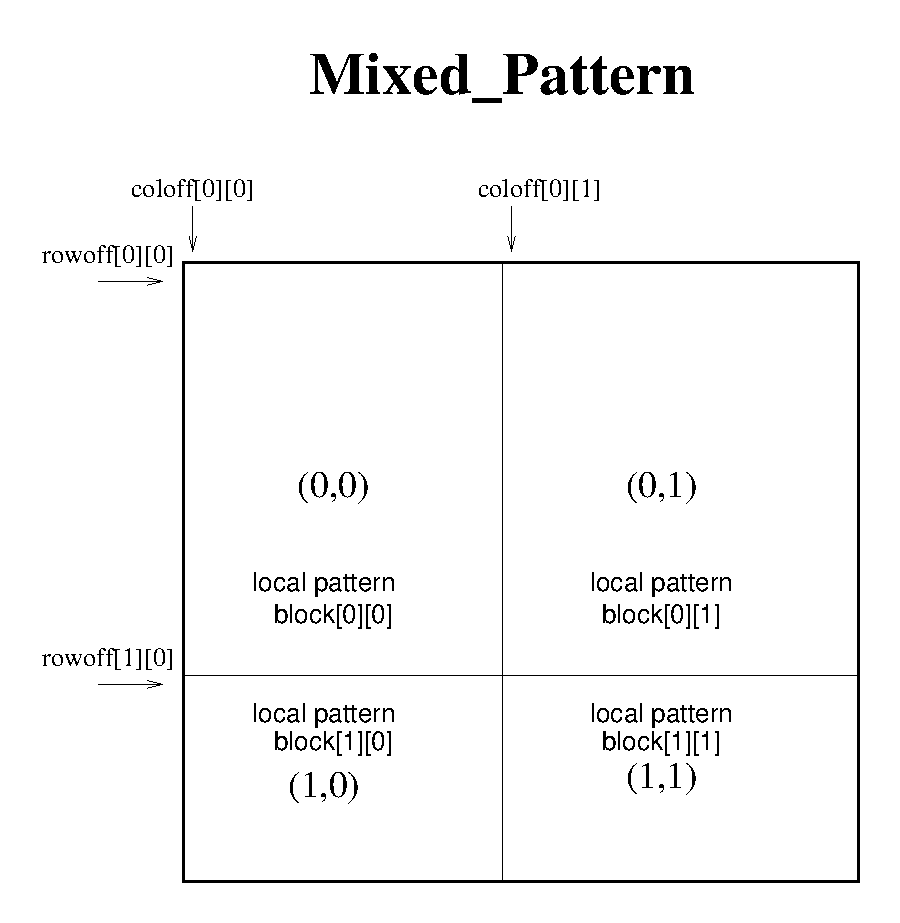
\includegraphics[width=0.7\textwidth]{mixed_pattern}
    
  \end{center}
  \caption{Schematic view of a $2\times2$ Mixed pattern}
\end{figure}

\subsection{The Basis Function class}
The \texttt{BasisFct} classes furnish the basis function for a finite
element and for a mapping and are defined in \texttt{basisFct.h}.  The
basic finite elements and the related node numbering are illustrated
in figure \ref{fig:fem}.
\begin{figure}[bp]
\begin{center}
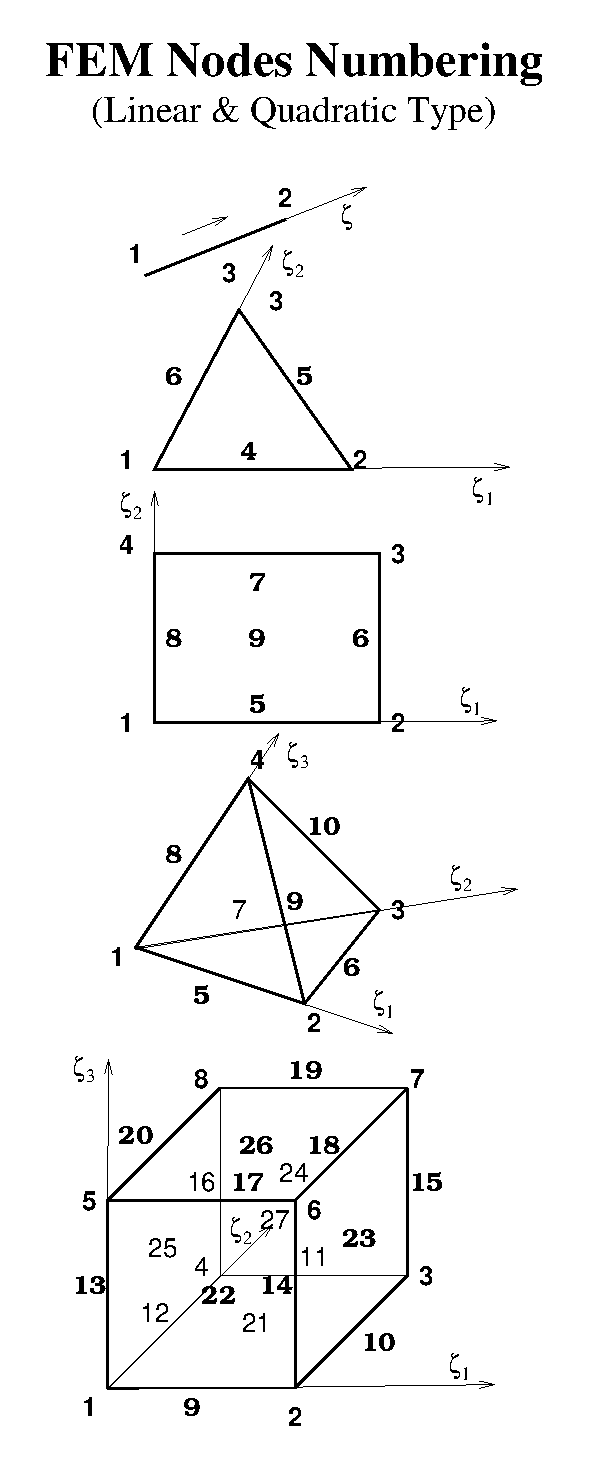
\includegraphics[height=.75\textheight]{Fem_nodes}
\end{center}
\caption{Finite element node numbering, both for linear and quadratic
  elements. Clearly, the lienar elements use only a subset of teh nodes
  here indicated. We use the general rule which imposes that the
  numbering follows the order: Vertices, Edges, Faces,
  Volumes (refer to figure \ref{fig:basrefsha})}\label{fig:fem}
\end{figure}

A \texttt{BasisFct} is basically a container of pointers to functions,
which define the shape function and their derivatives. At the time
being, only first derivatives have been considered, yet it may in
principle be possible to add more in the future.  The implementation
is rather simple (and a little tedious)
We start by defining a pointer to function type, to avoid exessive
typing later on:

\begin{verbatim}
typedef const Real & cRRef;
typedef Real (* Fct)(cRRef,cRRef ,cRRef);
\end{verbatim}
In order to simplify things we always use three arguments, even if
the function is the shape function of a 2D element (or even a 1D one).
Following a common procedure we start by defining a common interface
which will then be specialised by deriving the actual classes
It is a class template whose template arguments are a BasRefSha (see
section \ref{sec:basgeosha}) and an integer which indicates the number
of shape functions. The use of a template argument for 
the number of shape functions allow to instantiate at compile time a 
vector of pointers to function. In this way we have a more efficient code
and also a simpler constructor (indeed we use just the standard constuctor).

\begin{verbatim}
template<typename BRS,UInt _nbFct>
class BasisFct_Base
{
public:
  static const UInt nbCoor = BRSE::S_nDimensions;/* For Compatibility
                                          the name will be made uniform */
  static const UInt nbFct  = _nbFct; // Numero of Shape Functions
  typedef BRS BasRefSha; // Basic Reference Shape.
  Real fct(const UInt i,cRRef x,cRRef y, cRRef z) const;
  Real fctDer(const UInt i,const UInt icoor,cRRef x,cRRef y,cRRef z) const;
};
\end{verbatim}

\begin{tabularx}{\textwidth}{lX}
\hline
\texttt{nbCoor}& The number of coordinates. This variable is kept for
compatibility only, since now this datum is available through
the BasRefSha, and will be taken away soon.\\
\texttt{nbFct} & Number of Shape Functions. The template parameter
is made visible.\\
\texttt{BasRefSha} & The  Basic Reference Shape type. The template parameter
is made visible.\\
\texttt{fct} & value of the $i$-th shape function at \emph{reference coordinates} $(x,y,z))$;\\
\texttt{fctDer} & $icoor$ component ($1,2$ or $3$)
of the $i$-th shape function derivative at \emph{reference coordinates} $(x,y,z))$. \\
\hline
\end{tabularx}
The rest of the file is the public interface for the various
\texttt{BasisFct} classes, which implements the various 
finite elements. The details of the shape function definition may be found
in the header file, here we report only the class declarations (the ones
implemented so far). We signal here that the assigment of the
function pointers to the correct shape functions (which are defined as global
functions), is made by the class constructor. It is possible to define the functions
without resorting to a global declaration, but it does not give any practical advantage
(if not avoiding name clashes).

\begin{verbatim}
*/
class BasisFct_Q1_2D:     // Q1
  public BasisFct_Base<Quad,4>
{

};
class BasisFct_Q2_2D:     // Q2
  public BasisFct_Base<Quad,9>
{

};

class BasisFct_P1_3D:     // P1
  public BasisFct_Base<Tetra,4>
{

};

class BasisFct_P2_3D:     // P2
  public BasisFct_Base<Tetra,10>
{

};
\end{verbatim}
Clearly the list is still short, but it will be incrased with time.
\subsection{The geomap classes}
Another building block for the finite element class is the mapping.
The \texttt{geoMap.h} header file contains a prototype of the mapping
classes. 

This set of classes define the mapping between the actual and the
reference finite element. In particular, for domain elements
they should provide the methods for
computing
\begin{itemize}
\item The correpondance $\boldsymbol{\zeta}\to\mathbf{x}$ between
reference and actual coordinates;
\item The jacobian matrix of the mapping and its determinant.
\end{itemize}
For a boundary element the classes should provide
\begin{itemize}
\item The correpondance $\hat{\boldsymbol{\zeta}}\to\mathbf{x}$ between
reference and actual coordinates;
\item The derivatives of the mapping $\frac{\partial{\mathbf{x}}}{\boldsymbol{\zeta}}$;
\item The normal $\hat{\boldsymbol{\zeta}}\to\mathbf{n}(\boldsymbol{\zeta})$;
\item The ratio between elementary surface areas.
\end{itemize}

\textsl{Luca Note: There is still some work to do in order to provide a
  full set of estensible mapping classes, may be non necessarily based
  on a finite element type mapping (details may be found in the comments
  inside the header file).  Also the internal organisation should be
  changed to make the classes more flexible.  Furthermore, there is the
  need to define the mapping for a boundary element.  Anyway, we here
  present the classes public interface as it is at the moment, which is
  already a very good and powerful starting point. $\bullet$}

 
A \texttt{GeoMap} is a class template with arguments a quadrature rule
(\texttt{QuadRule}) a basis function (\texttt{BasisFct}) and a geometry
element (\texttt{GeoEle}).  The reason why we specify the quadrature
rule is the the GeoMap needs to store some array with the value of the
shape function and derivatives (provided by the \texttt{BasisFct}) at
quadrature point, in order to have them ready all the time. The
\texttt{GeoEle} is the geometry element (see section
\ref{sec:meshhandler}) on which a \texttt{Geomap} object is updated.
The idea is in fact that there is only one instance of \texttt{Geomap}
which is updated by passing the geometry data of a specific element.


\begin{verbatim}
template<class QuadRule,class BasisFct,class GeoEle>
class GeoMap
/*
|   #Prerequisites
|   BasisFct:nbFct must be less than equal Geoele::S_numPoints
*/
{
public:
  GeoMap();
  typedef          GeoEle      typeGeoEle;
  typedef          BasisFct    typeBasisFct;
  typedef          QuadRule    typeQuadRule;
  static const UInt nbMapNodes= BasisFct::nbFct;
  static const UInt nbCoor    = BasisFct::nbCoor;
  static const UInt nbQuadPt  = QuadRule::nbQuadPt;
\end{verbatim}
As usual, some template argument type and variables are 
brought at the level of the classes, to avoid using
name scope operators.

\begin{verbatim}
  void update(const GeoEle& geoele);
  void coorMap(Real& x,Real& y,Real& z,
               const Real & xi,const Real & eta, const Real &
               zeta) const; //(x,y,z) = F(xi,eta,zeta)
  void calcDetJac(Real det[nbQuadPt]);
  void calcDetInvJac(Real tInvJac[nbCoor][nbCoor][nbQuadPt],Real det[nbQuadPt]);
};
\end{verbatim}
\begin{tabularx}{\textwidth}{lX}
  \hline \texttt{update}& It takes a geometric element constant
  reference and updates he mapping on that element.It means that the
  successive calls to the class methods use the geometrical
  information of that element.\textbf{The user is warned that calling
    one of the other methods of the class without having
    \emph{update}d the \texttt{GeoMap} object gives unpredictable results}.\\
  \texttt{coorMap} & The map.\\
  \texttt{calcDetJac} & Returns the jacobian determinant at
  quadrature points. It uses and array.;\\
  \texttt{calcDetInvJac} & Inverse jacobian and its determinant at
  quadrature  points.  \textsl{Luca Note: I think that we should avoid using
    multidimensional native C++ arrays, because they are very error
    prone. We should give a closer look
    at the valarray classes of the STL.}\\
  \hline
\end{tabularx}
Now some global typedefs are created to make life easier.

\begin{verbatim}
typedef
GeoMap<QuadRule_Tetra_4pt,BasisFct_P1_3D,MeshElementMarked3D<LinearTetra> >
GeoMap_Linear_Tetra_4pt;
typedef
GeoMap<QuadRule_Tetra_1pt,BasisFct_P1_3D,MeshElementMarked3D<LinearTetra> >
GeoMap_Linear_Tetra_1pt;
typedef
GeoMap<QuadExact,BasisFct_P1_3D,MeshElementMarked3D<LinearTetra> >
GeoMap_Linear_Tetra_Exact;
typedef
GeoMap<QuadRule_Tetra_4pt,BasisFct_P2_3D,MeshElementMarked3D<QuadraticTetra> >
GeoMap_Quadratic_Tetra_4pt;
typedef
GeoMap<QuadRule_Tetra_1pt,BasisFct_P2_3D,MeshElementMarked3D<QuadraticTetra> >
GeoMap_Quadratic_Tetra_1pt;
\end{verbatim}
The name of the types follws the pattern
\begin{center}
\mbox{\texttt{GeoMap\_}$Fetype$\texttt{\_}$n$\texttt{pt}},
\end{center}
where $Fetype$ is the finite element type, such as \texttt{Linear\_Tetra}
and $n$ is the number of quadrature points.
The \texttt{QuadRule} template arguments (such as \texttt{QuadRule\_Tetra\_4pt})
are types defined in \texttt{quadRule.h} (see \ref{sec:quadrule}).

The type \texttt{GeoMap\_Linear\_Tetra\_Exact} is used to specialise the
\texttt{GeoMap} in case of exact integration (\textsl{Not by Luca: this
part is still to be done}).
\subsection{Quadrature Rules}
\label{sec:quadrule}
This template class contained in the header file \texttt{quadRule.h},
provide the data for numerical integration.
It has two template parameter, a \texttt{BasRefSha} (Basis Reference Shape, 
see section \ref{sec:basgeosha}), and an unsigned integer which defines the number of quadrature
points. It is a template parameter to allow static dimensioning of the arrays storing
the weight and quadrature points (to enhance efficiency). The actual implementation of
the class is done by \textit{specialised constructors}\cite{Stroustrup:2000}.
Here teh class public interface: 

\begin{verbatim}
template<typename BasRefSha, unsigned int _nbQuadPt>
class QuadRule
{
public:
  QuadRule();
  static const UInt nbQuadPt = _nbQuadPt;
  static const UInt nbCoor   = BasRefShaE::S_nDimensions;
  // For sake of simplicity it returns 0 if we are asking a coordinate
  // outide the scope of the Basis REference Shape 
  // (for example the z coordinate for a triangle)
  Real const & quadPtCoor(UInt const ig,UInt const icoor) const; 
  // It returns a pointer to an array containing the quad point
  // coordinate
  Real const * quadPtCoor(UInt const ig) const;
  Real const & weight(UInt const ig) const;
};
\end{verbatim}
\begin{tabularx}{\textwidth}{lX}
  \hline \texttt{nbQuadPt} & Number of quadrature points. As usual
  template arguments are
  brought to surface and made public.\\
  \texttt{nbCoor} & The dimension of the geometric figure identified
  by the
  \texttt{BasRefSha}.\\
  Real const \texttt{quadPtCoor} & $icoor$ coordinate of the $ig$-th
  quadrature point (starting from $1$). For sake of simplicity it
  returns 0 if we are asking a coordinate outiside the range
  $[1,\text{\texttt{nbCoor}}]$
  (for example the $3^{\text{rd}}$ coordinate for a triangle)\\
  Real const * \texttt{quadPtCoor} & Overloaded version which returns
  the whole
  quadrature point array for point \texttt{ig}.\\
  \texttt{weight} & The $ig$-th point weight.\\
  \hline
\end{tabularx}
We have defined a \textbf{dummy} class template as a partial specialisation
of the general class template, to be used  for exact integration. 
The idea is to keep the class notation consistent and implement exact integration
by template specialisation.
\begin{verbatim}
template<typename BasRefSha>
class QuadRule<BasRefSha,0>
{
public:
  static const UInt nbQuadPt = 0;
  static const UInt nbCoor   = BasRefShaE::S_nDimensions;
  Real const & quadPtCoor(UInt const ig,UInt const icoor) const 
    {return nbQuadPt;};
  Real const * quadPtCoor(UInt const ig) const {return 0;};
  Real const & weight(UInt const ig) const {return 0;};
};
\end{verbatim}

As usual, we use type definitions to save the user to remember all template
parameters.
\begin{verbatim}
typedef QuadRule<Quad,1> QuadRule_Quad_1pt;
typedef QuadRule<Quad,4> QuadRule_Quad_2pt;
typedef  QuadRule<Quad,9> QuadRule_Quad_3pt;
typedef QuadRule<Tetra,0> QuadRule_Tetra_Exact;
typedef QuadRule<Tetra,1> QuadRule_Tetra_1pt;
typedef QuadRule<Tetra,4> QuadRule_Tetra_4pt;
\end{verbatim}
Their meaning is evident.
\subsection{Finite Element Classes}
The actual finite elements classes are build it three  step. 
\begin{enumerate}
\item  In the first 
step we define the \emph{\ix{Base Finite Element}}
classes, which are concrete classes (no template) which contains the basis information about 
the degrees of freedom of a class of finite elements. In particular it contains the
indication of the association of the elemental degrees of freedom with the geometrical items
(see Paradigms, section \ref{sec:paradigms}) and the \emph{local matrix pattern}.
Their name ends in \texttt{\_Base}, to indicate that they are still \emph{Base} finite elements,
i.e.\  the data there contained still refer to the reference element.
\item The \texttt{FeDef} class template, is an intermediate class
  template where a \texttt{GeoMap}, a Base Finite Element  and
  a \texttt{quadRule} are put together to form an actual \emph{finite
    element definition}. The reason why this is not the ultimate finite
  element class is related to the fact that we wish to support mixed
  finite elements. An efficient handling of mixed finite element
  within the framework chosen for the library requires to define this
  intermediate class.
\item The \texttt{FiniteElement} class, which completes all the data of
  a \texttt{FeDef} with the tools for computing the elemental matrices.
\end{enumerate}



The \texttt{feDef.h} header file contains the Base Finite Element and
the FeDef classes.  Here an example taken from the header file:
\begin{verbatim}
class FE_P1_Tetra_Base
{
 public:
  typedef BasisFct_P1_3D BasisFct; // The Shape Functions.
  //
  static const UInt  nbNode       = BasisFct::nbFct;
  static const UInt  nbCoor       = BasisFct::nbCoor;
  //
  // Dof Information
  //
  static const UInt  nbDofPerVertex  = 1;
  static const UInt  nbDofPerEdge    = 0;
  static const UInt  nbDofPerFace    = 0;
  static const UInt  nbDofPerVolume  = 0;
  // 
  //Pattern Information
  //
  static const UInt  nbPattern    = nbNode*nbNode;
  static const UInt  nbDiag       = nbNode;
  static const UInt  nbUpper      = nbNode*(nbNode-1)/2;
  //
  static UInt patternFirst(const UInt i);
  static UInt patternSecond(const UInt i);
};
\end{verbatim}
\begin{tabularx}{\textwidth}{lX}
  \hline \texttt{BasisFct} & Generic typename which indicates the
  Basis Shape Function class used by the finite element.\\
  \texttt{nbCoor} & The dimension of the associated geometrical element
  (taken from the \texttt{BasisFct})\\
  \texttt{nDofPrrVertex} & The number of degrees of freedom attributed
  to a \texttt{Vertex} of the associated geometrical element.
  \textbf{Beware:} the number of degrees of freedom associated to a
  geometry entity is related to the order of the finite element, and are
  invariant to the fact that we are treating a scalar or a vector
  problem. In other words, a linear triangle will always have one one
  degree of freedom per vertices, also when used to solve a vector
  problem.
  Moreover, we are here talking of \texttt{Vertices}, \textbf{not Points!}.\\
  \texttt{nbDofPerEdge}& The number of degrees of freedom attributed to
  an \texttt{Edge} of the associated geometrical element. Beware that
  the Dof
  associated to the Edge ends are indeed DofPerVertex!\\
  \texttt{nbDofPerFace}&The number of degrees of freedom attributed to
  an \texttt{Face} of the associated geometrical element.\\
  \texttt{nbDofPerVolume} &The number of degrees of freedom attributed
  to the \texttt{Volume} geometrical element. Beware: this are the
  number of Dof ``internal'' to the volume, \textbf{not} the total
  number of Dof of the element.  \\
\texttt{nbPattern} & Number of elements
  of the local matrix, usually equal to \texttt{nbNode*nbNode}
  (\textsl{Luca Note: Indeed we may think of a
    generic pattern class, to be used for the standard cases});\\
  \texttt{nbDiag} & Number of diagonal terms in the local matrix,
  Usually equal to \texttt{nbNode} (\textsl{See previous note}); \\
  \texttt{nbUpper} & Number of terms in the upper triangula part of the
  local matrix;\\
  \texttt{patternFirst}& First term of the $i$-th element of the pattern ;\\
  \texttt{patternSecond}&Second term of the $i$-th element of the pattern.\\
  \hline
\end{tabularx}

\emph{Patterns} are organised so that the first local matrix element stored are
those on the diagonal, then the remaining terms 
are sorted (consequently the  lower triangular terms are first than the upper triangular ones);
The pattern data will be obviously used for the build-up of teh global matrices

We now give a closer look to the \texttt{feDef}: 
\begin{verbatim}
template <typename GM, typename BFE>
class FEDef : public BFE
{
public:
  typedef  typename GM::typeQuadRule QuadRule;/* Quadrule by GeoMap, 
                                        to ensure consistency:
                                        (TODO) to be done better! */
  typedef GM  GeoMap;
  typedef typename GeoMap::typeGeoEle   GeoEle;
  static const UInt  nbQuadPt     = QuadRule::nbQuadPt;
};
\end{verbatim}
It may be noticed that it is a class template which puts together the
basic ingredients of a finite element. The quadrule is not indicated
becouse it is implicitely defined by the mapping (\textsl{Luca Note:
  This is something that will be changed later on})
Finally, the header file provides some types (only a few, a lot more
will be added!)

\begin{tabularx}{\textwidth}{>{\ttfamily}lX}
  \hline 
FE\_P1\_Tetra\_1pt&  P1 Tetra finite element, 1 point of quadrature.\\
FE\_P1\_Tetra\_4pt&  P1 Tetra finite element, 4 point of quadrature.\\
FE\_P1\_Tetra\_Exact& P1 Tetra finite element, Exact quadrature.It
\textbf{MUST} be specialised, and that is done in the
\texttt{fe\_p1\_3d.h} header file.\\
FE\_P2\_Tetra\_1pt&  P2 Tetra isoparametric finite element, 1 point of quadrature.\\
FE\_P2\_Tetra\_4pt&  P2 Tetra isoparametric finite element, 4 point of quadrature.\\
FE\_P2\_Linear\_Tetra\_1pt&P2 Tetra affine finite element, 1 point of quadrature.\\
FE\_P2\_Linear\_Tetra\_4pt&P2 Tetra affine finite element, 4 point of
quadrature.\\
\hline
\end{tabularx}
\medskip


Finally, we look at the public interface of the template class in the \texttt{finiteEle.h}
header file
\begin{verbatim}
enum DerivSwitch {Measure,FirstDeriv,SecondDeriv};

//======================================================================
//
//                        Finite Element
//
//======================================================================
template<class FE>
class FiniteEle: 
  public FE
{
public:
  FiniteEle();
  //
  static const UInt nbDerivSwitch=3;
  bool getDerivSwitch(const DerivSwitch _s) const;  
  UInt currentID() const;
  void globCoorQuadPt(Real& x,Real& y,Real& z,const UInt ig) const;
  void update(const typename FE::GeoEle & geo_ele,const DerivSwitch d_sw=FirstDeriv);

  Real measure();
  void mass(Real* mat,const Real coef) const;
  void stiff(Real* mat,const Real coef) const;

  void source(Real* vec,const Real constant) const;
  template<class UsrFct> void source(Real* vec,const UsrFct& fct) const;
};
\end{verbatim}
This class template will be the basic block fo r\textbf{user defined
  finite element classes}. The \texttt{DerivSwitch} is a Switch (see
header file \texttt{switches.h}) which is used to indicate the 
type of data at quadtrature points the finite element builds when
it is \texttt{update}d on an actuale geometrical element.

\subsection{The specialised versions for exact integration}
\subsection{The Mixed finite element classes}

\subsection{The Degrees of Freedom}
\label{s:dof}
\subsection{The Fields}
\subsection{The assembly process}

%
%%%%%%%%%%%%% Some Settings for emacs and auc-TeX
% Local Variables:
% TeX-master: t
% TeX-command-default: "PDFLaTeX"
% TeX-parse-self: t
% TeX-auto-save: t
% x-symbol-8bits: nil
% TeX-auto-regexp-list: TeX-auto-full-regexp-list
% eval: (ispell-change-dictionary "american")
% End:
%

\chapter{HOWTO}

\section{Geometrical mappings}

In file \texttt{geoMap.h}:
 
GeoMap         : analytical mapping for parametric Lagrangian map
 
GeoMapQuadRule : derived from GeoMap when a quadrature rule is given 
  
GeoMap is the base class, two kinds of classes can be derived from it:

\begin{itemize}
\item GeoMapQuadRule : when a quadrature rule is used
\item various classes when an "exact" integration is used
\end{itemize}
 

\section{HOWTO add new basis functions}

The basis functions may be used  to define the geometrical mappings and
the finite element shape functions. A lot of basis functions are already
implemented in the file \verb#basisFct.h#. To create a new set of basis 
functions you must create a class which derives from the class 
{\verb BasisFct_Base<Shape,nbFct>}, where Shape is either Line or 
Quad or Triangle or Tetra or Hexa, and nbFct is the number of basis functions.
Your class has just to contain a constructor which fills the arrays fct[i] 
($0\leq i < nbFct$), and fctDer[i][icoor], ($0\leq i < nbFct$ and 
$0<icoor<Shape::S_nDimensions$). These arrays contain pointers to the basis
functions and their derivatives. These function are staightforwardly
coded as global function which take the coordinates $x,y,z$ as 
arguments and return the value of the function (see examples in the file   
\texttt{basisFct.h} ).

\section{HOWTO add a new quadrature rule}

The way is very similar to the one described for the basis
functions. You have just to derive a new class from the class
{\verb QuadRule<Shape,nbQuadPt>}. See the file \texttt{quadRule.h}

\section{HOWTO add a new element operator}

By ``element operator'', we mean element matrix corresponding to
a \ixs{differential}{operator} \ix{operator}. For example, the element \ixs{stiffness}{operator} or \ixs{mass}{operator}
matrices.

$\bullet${\bf First case}: you use a quadrature rule. Just add your 
operator in the file \texttt{elemOper.h} by copying and modifying an
existent one (e.g. stiff or mass). By this way, the new operator will 
work with arbitrary general finite elements. 

$\bullet${\bf Second case}: if you want to code ``hardly'' (without
integration rule) the element matrix corresponding to your operator for
a given finite element, you must create a ``specialized'' finite
element. This may be much more efficient, but the new operator will work
only with this element.

\section{HOWTO build a new finite element}

In \texttt{feBase.h}: create a base class for the new element (copy,
paste and modify an existant one...), say {\verb FE_My_Tetra_Base}. The
following depends on what you want to do.

$\bullet${\bf First case}: you want to use a quadrature rule. The
advantage: you will straighforwardly inherit all the work already done
for the other finite elements (in particular the operators defined in
\texttt{elemOper.h}). The drawback: if your finite element has a low order,
the comptationnal cost may be  more expensive than with a
``specialized integration''.

- have a look at the end of the file \texttt{geoMap.h}, you will
  find many geometrical mapping together with integration rules. Choose
  one, say \verb#GeoMap_Linear_Tetra_4pt#. If you don't like the
  geometrical mappings already defined, you have to create a new one.
  Remember that a geomapQR class is the ``tensorial product'' (template
  in fact...) of a set of basis function (in this example,
  \verb#BasisFct_P1_3D#, see \texttt{basisFct.h}), a geometric element (here,
  MeshElementMarked3D<LinearTetra>, see \texttt{basisElSh.h}) and a quadrature
  rule (here, \verb#QuadRule_Tetra_4pt#, see \texttt{quadRule.h}).

- in \texttt{finiteEleQR.h}: create a typedef correponding to the
  ``product'' of your base finite element and the geomap:
\begin{verbatim}
typedef FiniteEleQR<FE_My_Tetra_Base,GeoMap_Linear_Tetra_4pt> FE_My_Tetra_4pt;
\end{verbatim}
  
  $\bullet${\bf Second case}: you don't want to use a quadrature rule.
  Advantage: probably more efficient. Drawback: you have to reimplement
  your own element operators. Create a \texttt{MyGeoMap} class where you
  can store some geometrical stuffs, and a class \texttt{MyFE} where you
  store what you want accordingly to you finite element. The job now
  consists in developping the \emph{specialized} operators. 
It should look like
\begin{verbatim}
template<>
void stiff<MyFE,MyGeoMap>(Real coef,ElemMat& elmat,const MyFE& fe,
const MyGeoMap& geo,int iblock=0,int jblock=0)
...

\end{verbatim}
Thanks to the specialization, as soon as you adopt the same interface
for your operator than those of \texttt{elemOper.h}, a code
that works with a ``general'' FE (i.e. with a quadrature rule)
will work without any change with your new element.

You can have a look at \verb#fe_p1_tetra_exact.h#. But I emphasize that 
this is just a test, and it should probably be improved (in particular,
the geometrical quantities stored in the geomap class...).


%
%%%%%%%%%%%%% Some Settings for emacs and auc-TeX
% Local Variables:
% TeX-master: "lifev-dev"
% TeX-command-default: "PDFLaTeX"
% TeX-parse-self: t
% TeX-auto-save: t
% x-symbol-8bits: nil
% TeX-auto-regexp-list: TeX-auto-full-regexp-list
% eval: (ispell-change-dictionary "american")
% End:
%


\bibliographystyle{plain}
\bibliography{lifev}

\printindex

\end{document}

%
%%%%%%%%%%%%% Some Settings for emacs and auc-TeX
% Local Variables:
% TeX-master: t
% TeX-command-default: "PDFLaTeX"
% TeX-parse-self: t
% TeX-auto-save: t
% TeX-auto-regexp-list: TeX-auto-full-regexp-list
% eval: (ispell-change-dictionary "american")
% End:
%
